%%
%% Copyright 2007, 2008, 2009 Elsevier Ltd
%%
%% This file is part of the 'Elsarticle Bundle'.
%% ---------------------------------------------
%%
%% It may be distributed under the conditions of the LaTeX Project Public
%% License, either version 1.2 of this license or (at your option) any
%% later version.  The latest version of this license is in
%%    http://www.latex-project.org/lppl.txt
%% and version 1.2 or later is part of all distributions of LaTeX
%% version 1999/12/01 or later.
%%
%% The list of all files belonging to the 'Elsarticle Bundle' is
%% given in the file `manifest.txt'.
%%

%% Template article for Elsevier's document class `elsarticle'
%% with numbered style bibliographic references
%% SP 2008/03/01

\documentclass[preprint,10pt,a4paper,5p,authoryear,twocolumn]{elsarticle}

%% Use the option review to obtain double line spacing
%% \documentclass[authoryear,preprint,review,12pt]{elsarticle}

%% Load custom macros
\usepackage{macros}

%% For including figures, graphicx.sty has been loaded in
%% elsarticle.cls. If you prefer to use the old commands
%% please give \usepackage{epsfig}

%% The amssymb package provides various useful mathematical symbols
\usepackage{amssymb}
%% The amsthm package provides extended theorem environments
%% \usepackage{amsthm}

%% The lineno packages adds line numbers. Start line numbering with
%% \begin{linenumbers}, end it with \end{linenumbers}. Or switch it on
%% for the whole article with \linenumbers.
%\usepackage{lineno}

%% Set the bibliography style to be apalike i.e. author, year citation
\bibliographystyle{apalike}
%% By default, elsarticle loads the natbib package with round parameter showing
%% round brackets in citations. This can be changed to sqaure by setting the
%% citestyle
\setcitestyle{square}

%% Chemistry formulae support
\usepackage[version=4]{mhchem}

%% This turns references into clickable hyperlinks.
\usepackage[bookmarks,
            colorlinks=true,
            linkcolor=black,
            citecolor=black,
            urlcolor=blue,
            linktocpage,
            pageanchor=true]{hyperref} %,colorlinks

%% The subcaption package is used for figure and table sub-captions
\usepackage[list=true,position=b]{subcaption}

%% For code
\usepackage{listings}
\lstset{basicstyle=\scriptsize}

%% For charts
\usepackage{pgfplots}
\usetikzlibrary{pgfplots.groupplots}
\pgfplotsset{compat=1.13}

\journal{IEEE Computer Graphics \& Applications}

%% Setting the path to where the images can be found
\graphicspath{ {images/} }

\begin{document}

\begin{frontmatter}
  \title{Cross-platform ubiquitous volume rendering using programmable shaders in
  VTK for scientific and medical visualization}

\author{Aashish Chaudhary\corref{cor1}}
\ead{aashish.chaudhary@kitware.com}

\author{Sankhesh J. Jhaveri\corref{}}
\ead{sankhesh.jhaveri@kitware.com}

\author{Alvaro Sanchez}
\ead{alvaro.sanchez@kitware.com}

\author{Lisa S. Avila}
\ead{lisa.avila@kitware.com}

\author{Kenneth M. Martin}
\ead{ken.martin@kitware.com}

\author{David Lonie}
\ead{david.lonie@kitware.com}

\author{Marcus D. Hanwell}
\ead{marcus.hanwell@kitware.com}

\author{Will Schroeder}
\ead{will.schroeder@kitware.com}

\address{Kitware, Inc., 28 Corporate Drive, Clifton Park, NY 12065, USA}
\cortext[cor1]{Corresponding Author}


  \begin{abstract}
\label{abstract}The Visualization Toolkit (VTK) is a popular cross-platform, open source
toolkit for scientific and medical data visualization, processing, and
analysis. It supports a wide variety of data formats, algorithms, and rendering
techniques for both polygonal and volumetric data. In particular VTK's volume
rendering module has long provided a comprehensive set of features such as
plane clipping, color and opacity transfer functions, lighting, and other
controls needed for visualization. However, due to VTK's legacy OpenGL backend
and its reliance on a deprecated API, the system did not take advantage of the
latest improvements in graphics hardware or the flexibility of a programmable
pipeline. Additionally, this dependence on an antiquated pipeline posed
restrictions when running on emerging computing platforms, thereby limited its
overall applicability. In response to these limitations, the VTK community
developed a new and improved volume rendering module, which not only produced
a modern GPU-based implementation, but also augmented its capabilities with new
features such as fast volume clipping, gradient magnitude based opacity
modulation, render to texture, and hardware-based volume picking.
\end{abstract}


  \begin{keyword}
    Visualization Toolkit \sep
    Data analysis \sep
    Volume rendering \sep
    Scientific Visualization \sep
  \end{keyword}
\end{frontmatter}

%\linenumbers

VTK has a long history of volume rendering and, unfortunately, that history is
evident in the large selection of classes available to render volumes. Each of
these methods was state-of-the-art at the time, but given VTK’s 20+ year
history, many of these methods are now quite obsolete. One of the goals of this
work is to reduce the number of volume mappers to ideally just two: one that
supports accelerated rendering on graphics hardware and another that works in
parallel on the CPU. The vtkSmartVolumeMapper would help application developers
by automatically choosing between these techniques based on system performance. 

\begin{figure}[h]
  \centering
  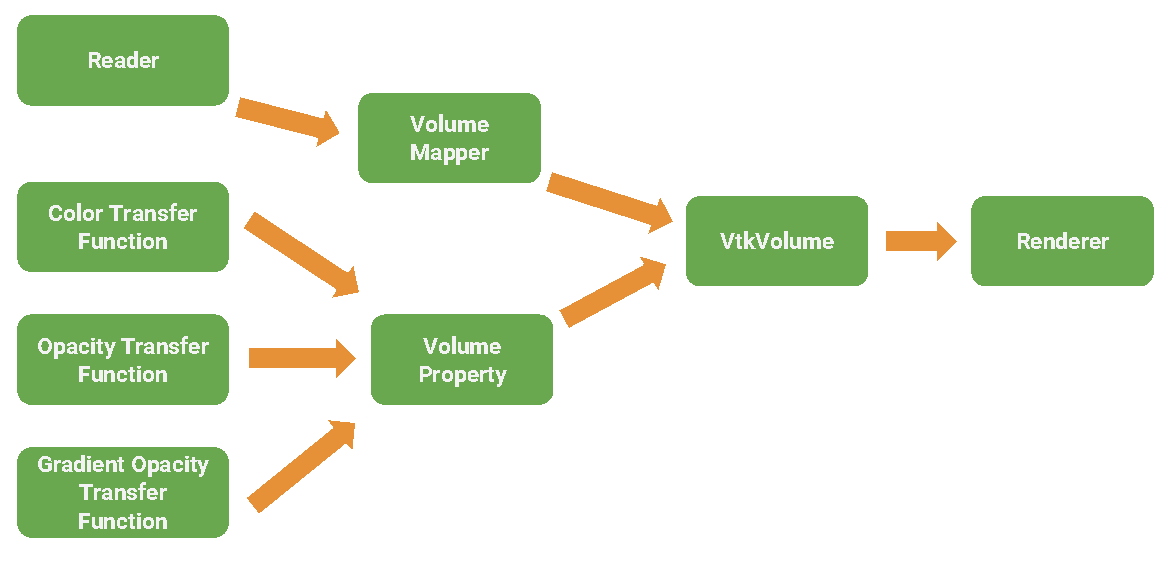
\includegraphics[width=\columnwidth]{vtk_volume_pipeline.pdf}
  \caption{VTK pipeline for volume rendering which is similar to VTK polygonal
    rendering with differences such as transfer functions are defined on the
    property object.}
  \label{fig:pipeline}
\end{figure}%

The main objective of this effort is to create a cross-platform,
multi-functional and high-performance volume renderer that works in both serial
and parallel mode (for example in
ParaView\cite{ahrens_paraview:_2005,ayachit_paraview_2015}). To achieve this,
we have created a replacement for the OpenGL fixed pipeline based
vtkGPUVolumeRayCastMapper. The new mapper, which shares the same name but uses
the OpenGL programmable pipeline, can be used via vtkSmartVolumeMapper or
instantiated directly and replaces the old vtkGPUVolumeRayCastMapper.
Availability of the new mapper with new OpenGL-VTK implementation improved the
management of textures in the mapper and benefited both forms of rendering
(geometry and volume) by sharing common code between them. While volume
ray-casting itself is a well-known technique, developing a volume renderer that
works with variety of data formats and types, supports many essential features
for medical and scientific computing, works on the main commercial platforms
(such as Windows, Mac, and Linux) and performs well at interactive frame rates
with very large datasets is still a challenging task that requires an in-depth
knowledge of the data, graphics pipeline, the VTK framework and the user
requirements.  In the next section, we will cover technical details of our work
that resulted in a sophisticated volume renderer for the VTK community.

\section{Related Work}
\label{relatedwork}

Volume Visualization enables viewing of three-dimensional data by rendering
sampled function of three spatial dimensions and projecting the translucent
volume onto a 2D projection plane. While many techniques exist for volume
rendering such as marching cubes~\citep{lorensen_marching_1987}, image
splatting~\citep{westover_footprint_1990}, texture
slicing~\citep{rezk-salama_interactive_2000, engel_high-quality_2001} and ray
casting~\citep{hsu_segmented_1993, ma_parallel_1995, ma_scalable_1997,
heng_gpu-based_2005}, ray casting has become one of the most used ones on modern
graphics hardware. Ray casting technique provides a higher quality of rendering
and many ways to optimize the rendering of the volume such as early ray
termination and space leaping~\citep{yagel_accelerating_1993}.

While the Ray Casting a well-known technique and various implementations exists,
the challenge of providing high-quality volume visualization with dataset of
varying size, spacing, and format, with or without the geometry rendering, on
multiple platforms (Desktop, Cave, Head Mounted Displays (HMD)) and Operative
Systems (Apple, Linux, Window) at interactive speed is still a challenge.

Few open-source implementations exist such as
Voreen~\citep{meyer-spradow_voreen:_2009} which initiated at Department of
Computer Science at the University of Münster, Germany in 2004.  It provides
features such as Isosurface Rendering, Maximum Intensity Projection
(MIP)~\citep{wallis_three-dimensional_1989}, support for 1D and 2D transfer
functions, and support for different illumination models (Phong, Tone, Ambient
Occlusion). Both Voreen and VTK uses data-flow networks. However, Voreen is
Volume Visualization library whereas VTK is a Scientific Visualization library
and provides better support for Geometry and Gridded datasets. While Voreen
provides a rapid prototyping environment, VTK volume visualization aims for
production quality, performance, and Ubiquitousness. Additionally, Voreen only
supports high-end desktop devices where as VTK supports multiple platforms
natively enabling researchers bridging the gap between academic research and
open source and industrial contributions.

Another open-source volume rendering ImageVis3D is being developed by the
researchers at the University of Utah~citep{SCI:ImageVis3D}. ImageVis3D is an
application as opposed to a library and provides support for large volume data
visualization, volume visualization on a desktop and mobile device, MIP, 1D and
2D transfer functions amongst many others.  It does not support Virtual Reality
environments and the flexibility of a data-flow networks.  Few other data type
specific volume rendering libraries such as Voxx~\citep{clendenon_voxx:_2002}
and ClearVolume~\cite{royer_clearvolume:_2015} provides visualization of
biological and light-sheet microscopy. PyMOL~\cite{schrodinger_llc_pymol_2015}
provide volume visualization capabilities only to molecular datasets. Finally,
hardware architecture specific volume visualiation libraries such as
OSPRay~\cite{wald_ospray_2017} and NVIDIA\textsuperscript{\textregistered}
Optix\textsuperscript{\texttrademark}~\citep{parker_optix:_2010} provide fast
large volume data visualization capabilities on Intel CPU and Nvidia GPU's but
lack support for non-native hardware.

Other than Voreen and ImageVis3D, many volumes rendering APIs exist, however,
except for Voreen, advanced volume visualization research performed by the
industry and academic communities are not publicly available. By providing an
open source volume rendering engine that supports multiple platforms natively,
researchers can use the engine as a bridge between academic research and open
source and industrial contributions.

\section{Implementation Details}
\label{implementationdetails}
The new~\texttt{vtkGPUVolumeRayCastMapper} uses a ray casting
technique~\citep{engel_real-time_2006} for volume rendering which is
state-of-the-art on modern graphics platforms. At a high level it is similar to
the previous version of this class, with a different OpenGL implementation
reflecting recent advances in graphics systems. One of the main reason we chose
to use ray casting due to the flexibility of this technique, which supports the
many features of the previous software ray cast mapper but with the acceleration
of the GPU. Ray casting is an image-order rendering technique, with one or more
rays cast through the volume per image pixel. VTK is inherently an object-order
rendering system, where the GPU renders all graphical primitives (points, lines,
triangles, etc.) represented by instances of vtkProp in a scene using one or
more rendering passes (with multiple passes needed to support advanced features
such as depth peeling for transparency).

The image-order rendering process for vtkVolume is initiated when the
front-facing polygons of the volume’s bounding box are rendered with a custom
fragment program. This fragment program is used to cast a ray through the volume
at each pixel, with the fragment location indicating the starting location for
that ray. The volume and all the various rendering parameters are transferred to
the GPU through the use of textures (3D for the volume, 1D for the various
transfer functions) and uniform variables. Steps are taken along the ray until
the ray exits the volume, and the resulting computed color and opacity are
blended into the current pixel value. Note that volumes are rendered subsequent
to rendering opaque geometry to allow the ray casting process to terminate at
the depth value stored in the depth buffer for that pixel (and, hence, correctly
intermix with opaque geometry).

In addition to providing supported features of the old mapper, the new mapper
adds new capabilities such as GPU-based clipping,  gradient opacity, and volume
picking amongst many others. In the next few sections, we will cover each of
these features in detail.

\subsection{Single Pass}
% \begin{figure}[ht]
%   \centering
%   
\includegraphics[width=\columnwidth]{frontandback.png}
%   \caption{Front and back faces are rendered for start and end position of the
%   ray.}
%   \label{fig:frontandback}
% \end{figure}%


% \begin{figure}[ht]
%   \centering
%   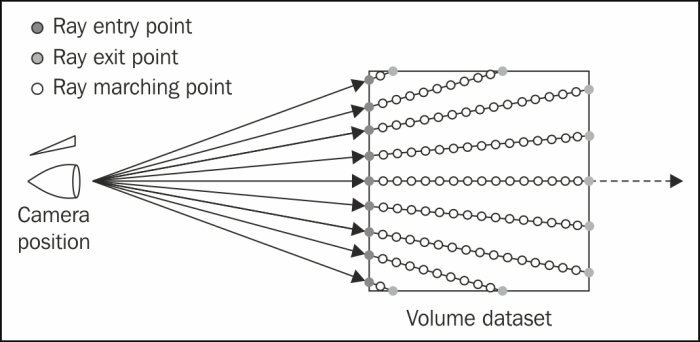
\includegraphics[width=\columnwidth]{raycasting}
%   \caption{Implementing volume rendering using single-pass GPU ray casting.}
%   \label{fig:raycasting}
% \end{figure}%

In a ray-casting algorithm, the entry and the exit point into the volume is
needed to determine when to stop ray stepping procecss. To determine the entry and
the exit point, one approach is to render the geometry of the volume bounding
box of the volume twice. In the first pass, the front face of the geometry is
rendered and in the second pass the backface is rendered.
% as shown in ~\Autoref{fig:frontandback}.
Using the interpolated vertex position and
texture lookup, the start and end positions can be computed. Instead of this, in
\texttt{vtkGPUVolumeRayCastMapper}, entry and exit points are computed based on
the fact that the texture extents of the volume are within vec3(1.0), vec3(-1.0)
range.% (as shown in ~\Autoref{fig:raycasting}).
The code below shows the
fragment shader pseudo code that determines whether or not to stop ray stepping
through the volume.

\begin{center}
  \begin{lstlisting}[language=Python, caption={Ray stop determination},
                     captionpos=b, frame=single, breaklines=true]
bool stop = any(greaterThan(g_dataPos,
                            ip_texMax)) ||
            any(lessThan(g_dataPos,
                         ip_texMin));
  \end{lstlisting}
\end{center}

The advantage of such approach is that it requires one less pass and is faster
than other approaches since there is no texture generation or lookup required
to determine the termination of the ray.


\subsection{Dynamic Shader Generation}
All operations are performed on the GPU in the
new~\texttt{vtkOpenGLGPUVolumeRayCastMapper}. The advantage of this approach is
more streamlined code that is easier to maintain and debug. This approach also
provides an opportunity to rework how to support different features without
having too many branches in the shader code or having to send all the options to
the shader because that would have been detrimental to the performance. In this
improved mapper, the shader is dynamically composed by the mapper. For this to
work, we have introduced tags in a vertex or fragment shader which are then
replaced by the~\texttt{vtkVolumeShaderComposer} depending on the options
enabled or chosen by the application code. These tags corresponds to each setup
in a ray casting shader: 1) Declaration of variables 2) Initialization of ray
position and direction 3) Iterative Ray traversal inside the volume and check
for ray termination conditions 4) Final color and opacity computation after ray
termination. For instance, the skeleton fragment shader defines tags as shown
in~\Autoref{lst:skeletonshader}.

\begin{lstlisting}[language=C++, caption={Fragment shader tags},
                   captionpos=b, frame=single, breaklines=true,
                   label=lst:skeletonshader]
//VTK::Base::Dec

//VTK::Termination::Dec

\end{lstlisting}

At runtime the \texttt{//VTK::Base::Dec} tag is replaced by shader code
shown in~\Autoref{lst:basedeclshader}

\begin{lstlisting}[language=C++, caption={Base declaration fragment code},
                   captionpos=b, frame=single, breaklines=true,
                   label=lst:basedeclshader]
// Volume dataset
uniform sampler3D in_volume;
uniform int in_noOfComponents;
uniform int in_independentComponents;

uniform sampler2D in_noiseSampler;
#ifndef GL_ES
uniform sampler2D in_depthSampler;
#endif

// Camera position
uniform vec3 in_cameraPos;

// view and model matrices
uniform mat4 in_volumeMatrix;
uniform mat4 in_inverseVolumeMatrix;
uniform mat4 in_projectionMatrix;
uniform mat4 in_inverseProjectionMatrix;
uniform mat4 in_modelViewMatrix;
uniform mat4 in_inverseModelViewMatrix;
uniform mat4 in_textureDatasetMatrix;
uniform mat4 in_inverseTextureDatasetMatrix;
varying mat4 ip_inverseTextureDataAdjusted;
uniform vec3 in_texMin;
uniform vec3 in_texMax;
uniform mat4 in_textureToEye;

// Ray step size
uniform vec3 in_cellStep;
uniform vec2 in_scalarsRange[4];
uniform vec3 in_cellSpacing;

// Sample distance
uniform float in_sampleDistance;

// Scales
uniform vec3 in_cellScale;
uniform vec2 in_windowLowerLeftCorner;
uniform vec2 in_inverseOriginalWindowSize;
uniform vec2 in_inverseWindowSize;
uniform vec3 in_textureExtentsMax;
uniform vec3 in_textureExtentsMin;

// Material and lighting
uniform vec3 in_diffuse[4];
uniform vec3 in_ambient[4];
uniform vec3 in_specular[4];
uniform float in_shininess[4];

// Others
uniform bool in_cellFlag;
uniform bool in_useJittering;
vec3 g_rayJitter = vec3(0.0);
uniform bool in_clampDepthToBackface;

uniform vec2 in_averageIPRange;
\end{lstlisting}

To define a structure, we have chosen a strategy that separates the tags in
the following four categories:

\begin{enumerate}
\label{enu:shadertags}
  \item \textbf{Declaration (::Dec)} The tags belonging to this group are meant
    to declare variables or function outside the main execution of the shader
    code.  The variables defined are uniform, varying, and user-defined global
    variables.  The functions defined are typically perform operations that are
    repetitive in nature such as computing color of a fragment.

  \item \textbf{Initialization (::Init)} The tags belonging to this group are
    meant to initialize variables inside the main execution function of the
    shader but before the ray-casting loop in the fragment shader. An example of
    such code includes computation of ray initial position and direction
    of traversal.

  \item \textbf{Implementation (::Impl)} The tags belonging to this group are
    the variables or functions or the combination of both that perform the
    actual operation of clipping, cropping, shading, etc. on one, two, or four
    component volume data.  The implementation code uses local and global
    variables and is optimized for performance reasons as it is executed as long
    as the ray is traversing inside the volume and didn't run into a termination
    condition which is checked every time.

  \item \textbf{Exit (::Exit)} The tags belonging to this group perform final
    computation such as the final color of the fragment. These tags are placed
    outside the ray-casting loop and typically contain numeric assignments.
\end{enumerate}

\subsection{Lighting / Shading}
\label{lighting}
The old mapper supported only one light (due to limitations in OpenGL at the
time the class was written). Similarly
the~\texttt{vtkFixedPointVolumeRayCastMapper} supports multiple lights, but only
with an approximate lighting model, since gradients are precomputed and
quantized, and shading is performed for each potential gradient direction
regardless of fragment location. However the new mapper accurately implements
the VTK lighting model to produce high quality images for publication. To
support this, depending on the light type (point, directional, and positional),
the lighting parameters are sent to the shader which then performs the per pixel
lighting calculations. The number of lights is limited to six mostly for
performance reasons as the interactive frame rate goes down significantly with
each light added to the scene. The Phong shading lighting model is used for
volume rendering lighting. Phong lighting requires normals which must be
computed for each fragment. The normal calculation is done by first computing
the gradient and then scaling the gradient by the spacing between the cells. The
gradient is computed by reading the scalar values form the neighboring cells
using the offset vector that stores the step size based on the bounds of the
volume.

\subsection{Volume Picking}
\label{picking}
Picking, in the context of volume rendering, is the action of resolving the set
of voxels a user has clicked on with the pointer. This provides the user with
means to interact with the objects in a 3D scene. VTK legacy volume mappers
support picking through an instance external to the mapper itself
called~\texttt{vtkVolumePicker}.  This class casts a ray into the volume and
returns the point where the ray intersects an isosurface of a user specified
opacity.  This technique has certain limitations given that the picking class
does not have enough information to correctly account for clipping, transfer
functions and other parameters defining how the mapper actually renders, thus
reducing its reliability on the actual objects being picked.

Now VTK supports hardware-accelerated picking of geometric data through the
class~\texttt{vtkHardwareSelector}, which uses a multiple-render-pass approach
in order to resolve the various objects in a scene (actors or props in VTK
parlance) and their corresponding primitives.  Each pass renders separately a
different selection abstraction (processes, actors, composite blocks and
primitives), painting with a different color each of the various components in
the scene.  The images rendered by each pass are downloaded from the GPU and
subsequently analyzed in the class thereby resolving the correspondence of each
pixel to its particular actor, primitive, etc.

The inherent flexibility of the revamped shader implementation of this mapper
permits a seamless integration with~\texttt{vtkHardwareSelector}'s interface by
rendering the appropriate colors for each of its passes, hence granting
consistency in the object selection regardless of whether it is geometric or
volumetric data.  Providing selection support directly within the fragment
shader ensures high selection accuracy even in situations where a volume
intermixes with geometry in seemingly cumbersome ways or other advanced features
(e.g. clipping) are enabled (what you see is what you pick).  Given the readily
available picking styles supported by~\texttt{vtkHardwareSelector}
(e.g.~\texttt{vtkAreaPicker}), it is possible to make a selection of a specific
set of visible voxels.

\subsection{Volume Texture Streaming}
\label{streaming}
A common limitation of volume rendering is that the 3D volume data does not
always fit into the graphics memory of a system. This limitation has become
increasingly important to address as the new mapper provides support for mobile
architectures.  A relatively simple method when dealing with a large volume is
the volume streaming approach also commonly known as
bricking~\citep{engel_real-time_2006} in which the volume is split into several
blocks so that a single sub-block (brick) fits completely into GPU memory.  Each
sub-block is stored in main memory and streamed into GPU memory for a rendering
pass one at a time (in a back-to-front manner for correct composition). The
sub-blocks are rendered using the standard shader programs and alpha-blended
with each other by OpenGL. Streaming the volume as separate texture bricks
certainly imposes a performance trade-off but acts as a graphics memory
expansion scheme for devices that are not able to render a large volume
otherwise.

\subsection{Dual Depth-Peeling}
\label{peeling}
VTK has long supported the use of depth-peeling for order-independent rendering
of translucent geometry. Since translucent fragments must be blended in a
specific order to obtain the correct pixel color, techniques like depth-peeling
are necessary for correctly shading a complex scene.

In a multipass depth-peeling rendering, `slices' of fragments are pulled from
the scene in depth order; the nearest fragments per pixel are collected in
the first pass, and then the fragments just behind those are written in the next
pass. After each pass, the current set of fragments is blended into an
accumulation buffer, ultimately producing a correctly colored scene in which all
fragments are blended from front-to-back.

The standard depth-peeling algorithm, which collects a single layer of fragments
per geometry pass in front-to-back order, was recently updated to use a ``dual
depth-peeling'' technique~\citep{bavoil_order_2008}, in which two layers of
fragments are peeled in a single geometry pass: One layer from the front and a
second from the back. These are blended into two separate accumulation buffers
and eventually the front and back peels will meet towards the middle of the
geometry. This allows depth-peeling to be carried out in roughly half as many
geometry passes.

An interesting detail of the new depth-peeling implementation is that there are
four depth values available per-pixel during a typical peeling pass. Two depth
values each are associated with the front and back peels; these are the depth of
the currently peeled fragment, and the depth of the next fragment that will be
peeled. These depth values can be reinterpreted as two sets of ``inner'' and
``outer'' boundaries for a view-ray traversing a volume.

By adapting the volume mapper's fragment shader to use these depth values for
computing two ``slices'' of a volume, we are able to integrate volume rendering
into our depth-peeling pass. This enables volumetric data to be mixed with
translucent geometry while efficiently yielding a correctly colored result
~\Autoref{fig:volume_peeling_tooth}.

\begin{figure}[ht]
\centering
  \begin{subfigure}[b]{.5\columnwidth}
    \centering
    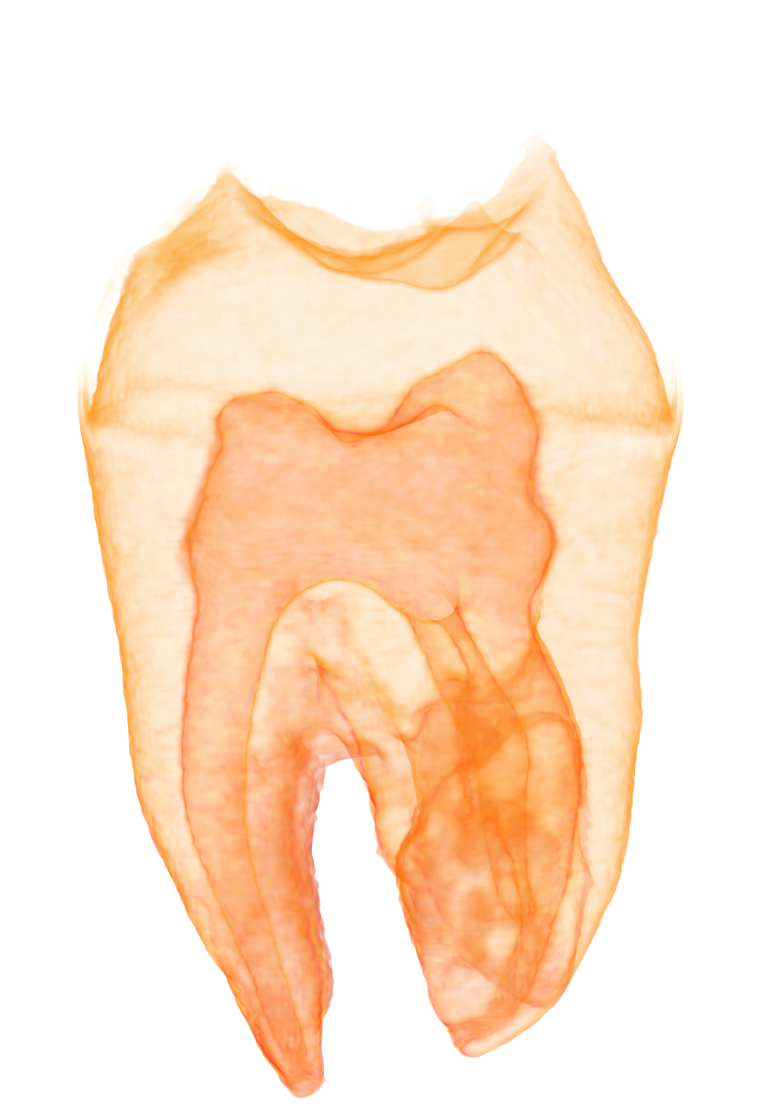
\includegraphics[width=\columnwidth]{tooth_front_}
    \caption{Volume only}
    \label{fig:tooth_front}
  \end{subfigure}%
  \begin{subfigure}[b]{.5\columnwidth}
    \centering
    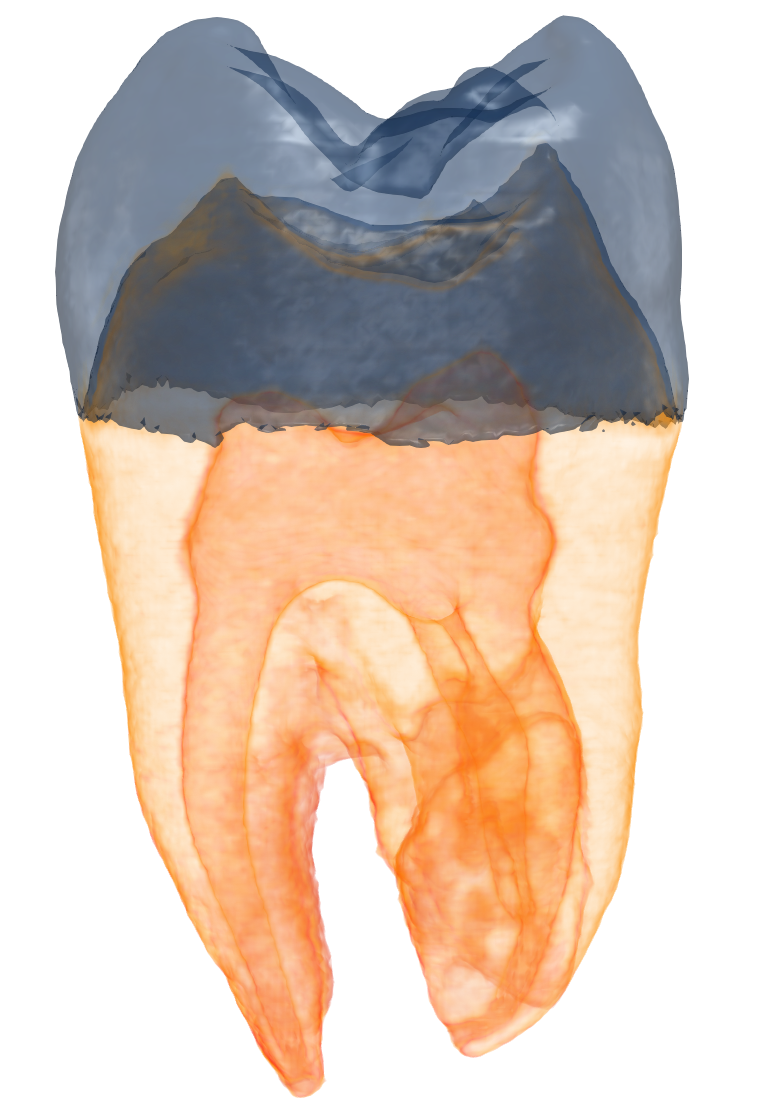
\includegraphics[width=\columnwidth]{tooth_front_enamel}
    \caption{Intermixed}
    \label{fig:tooth_front_enamel}
  \end{subfigure}
  \begin{subfigure}[b]{.5\columnwidth}
    \centering
    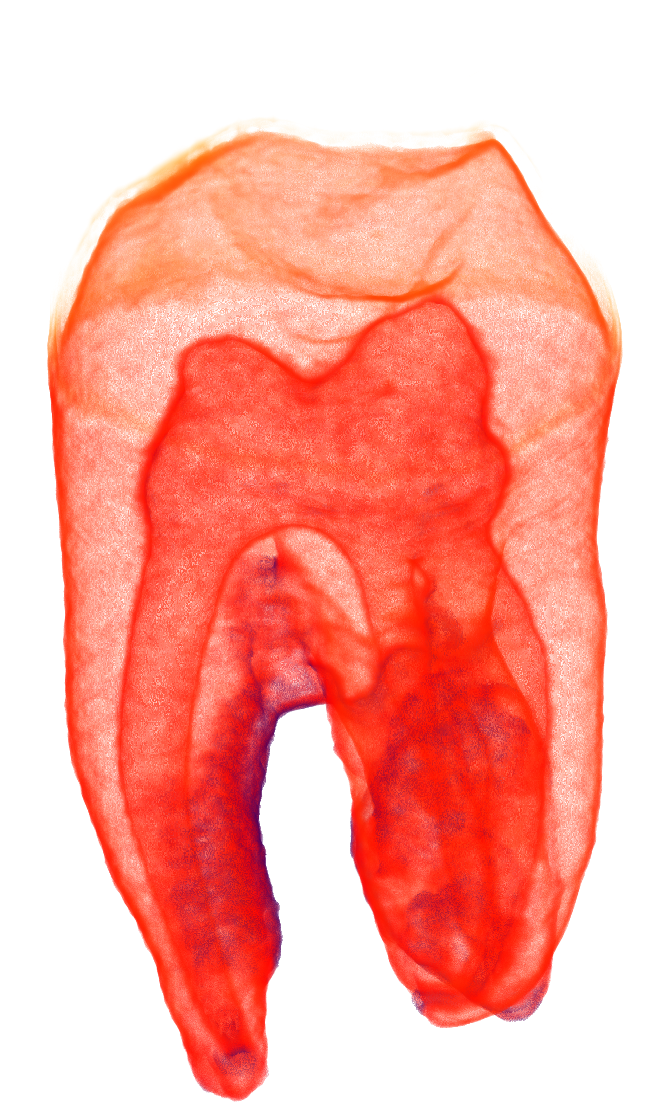
\includegraphics[width=\columnwidth]{tooth_bottom_}
    \caption{Volume only (rotated)}
    \label{fig:tooth_bottom}
  \end{subfigure}%
  \begin{subfigure}[b]{.5\columnwidth}
    \centering
    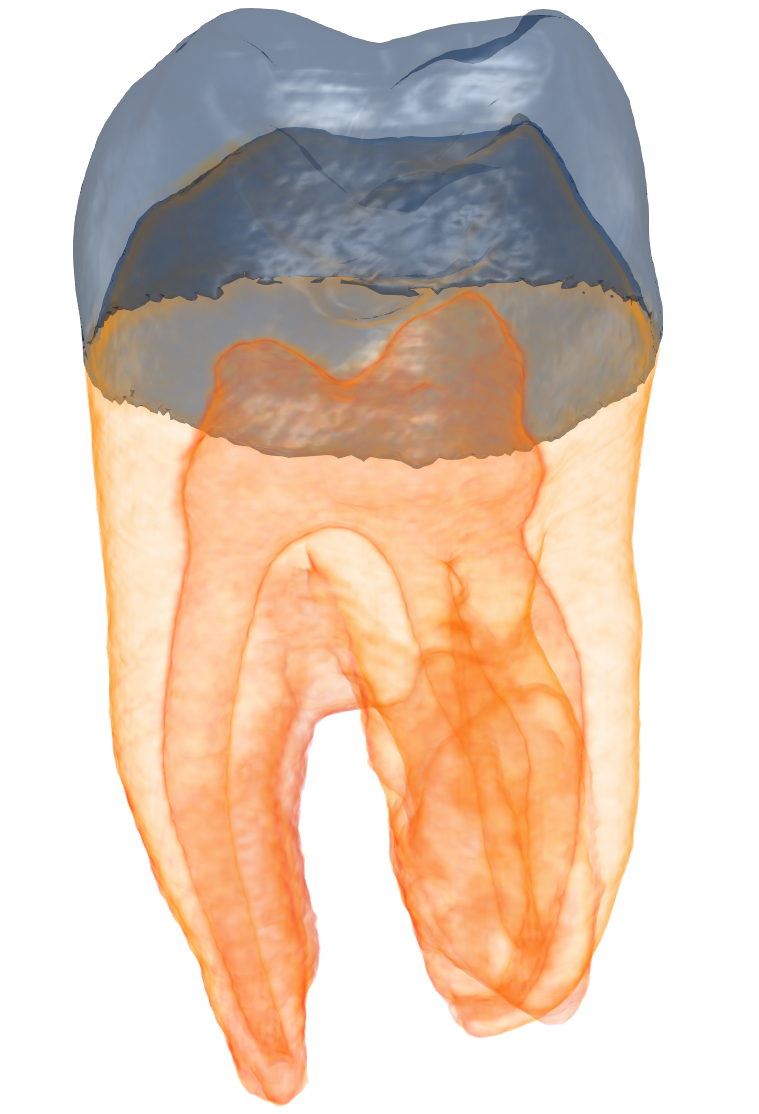
\includegraphics[width=\columnwidth]{tooth_bottom_enamel}
    \caption{Intermixed (rotated)}
    \label{fig:tooth_bottom_enamel}
  \end{subfigure}
  \caption{Industrial CT scan of a human tooth~\citep{pfister_transfer_2001}.
    The dentin and pulp of the tooth are rendered as a volume (a) while an
    iso-contour of the enamel is rendered as translucent polygonal geometry (b).
    (c) and (d) show a different viewpoint (object rotated on the horizontal axis)
    from which it is easier to observe the correct ordering of the rendered
    entities.}
  \label{fig:volume_peeling_tooth}
\end{figure}

\subsection{Render to Texture}
\label{rendertotexture}
Typically, the mapper uses a single pass
rendering approach in which the 3D volume data is rendered on screen i.e. the
default framebuffer that comprises of a color and a depth buffer. In games and
other graphics applications, a multi-pass rendering approach called ``Render to
Texture'' is used to support advanced visual rendering techniques such as
deferred shading, texture baking, post processing, etc. This technique uses the
rendered output from one pass to modify/enhance the output of another rendering
passes.

\begin{figure}[ht]
\centering
  \begin{subfigure}[b]{.5\columnwidth}
    \centering
    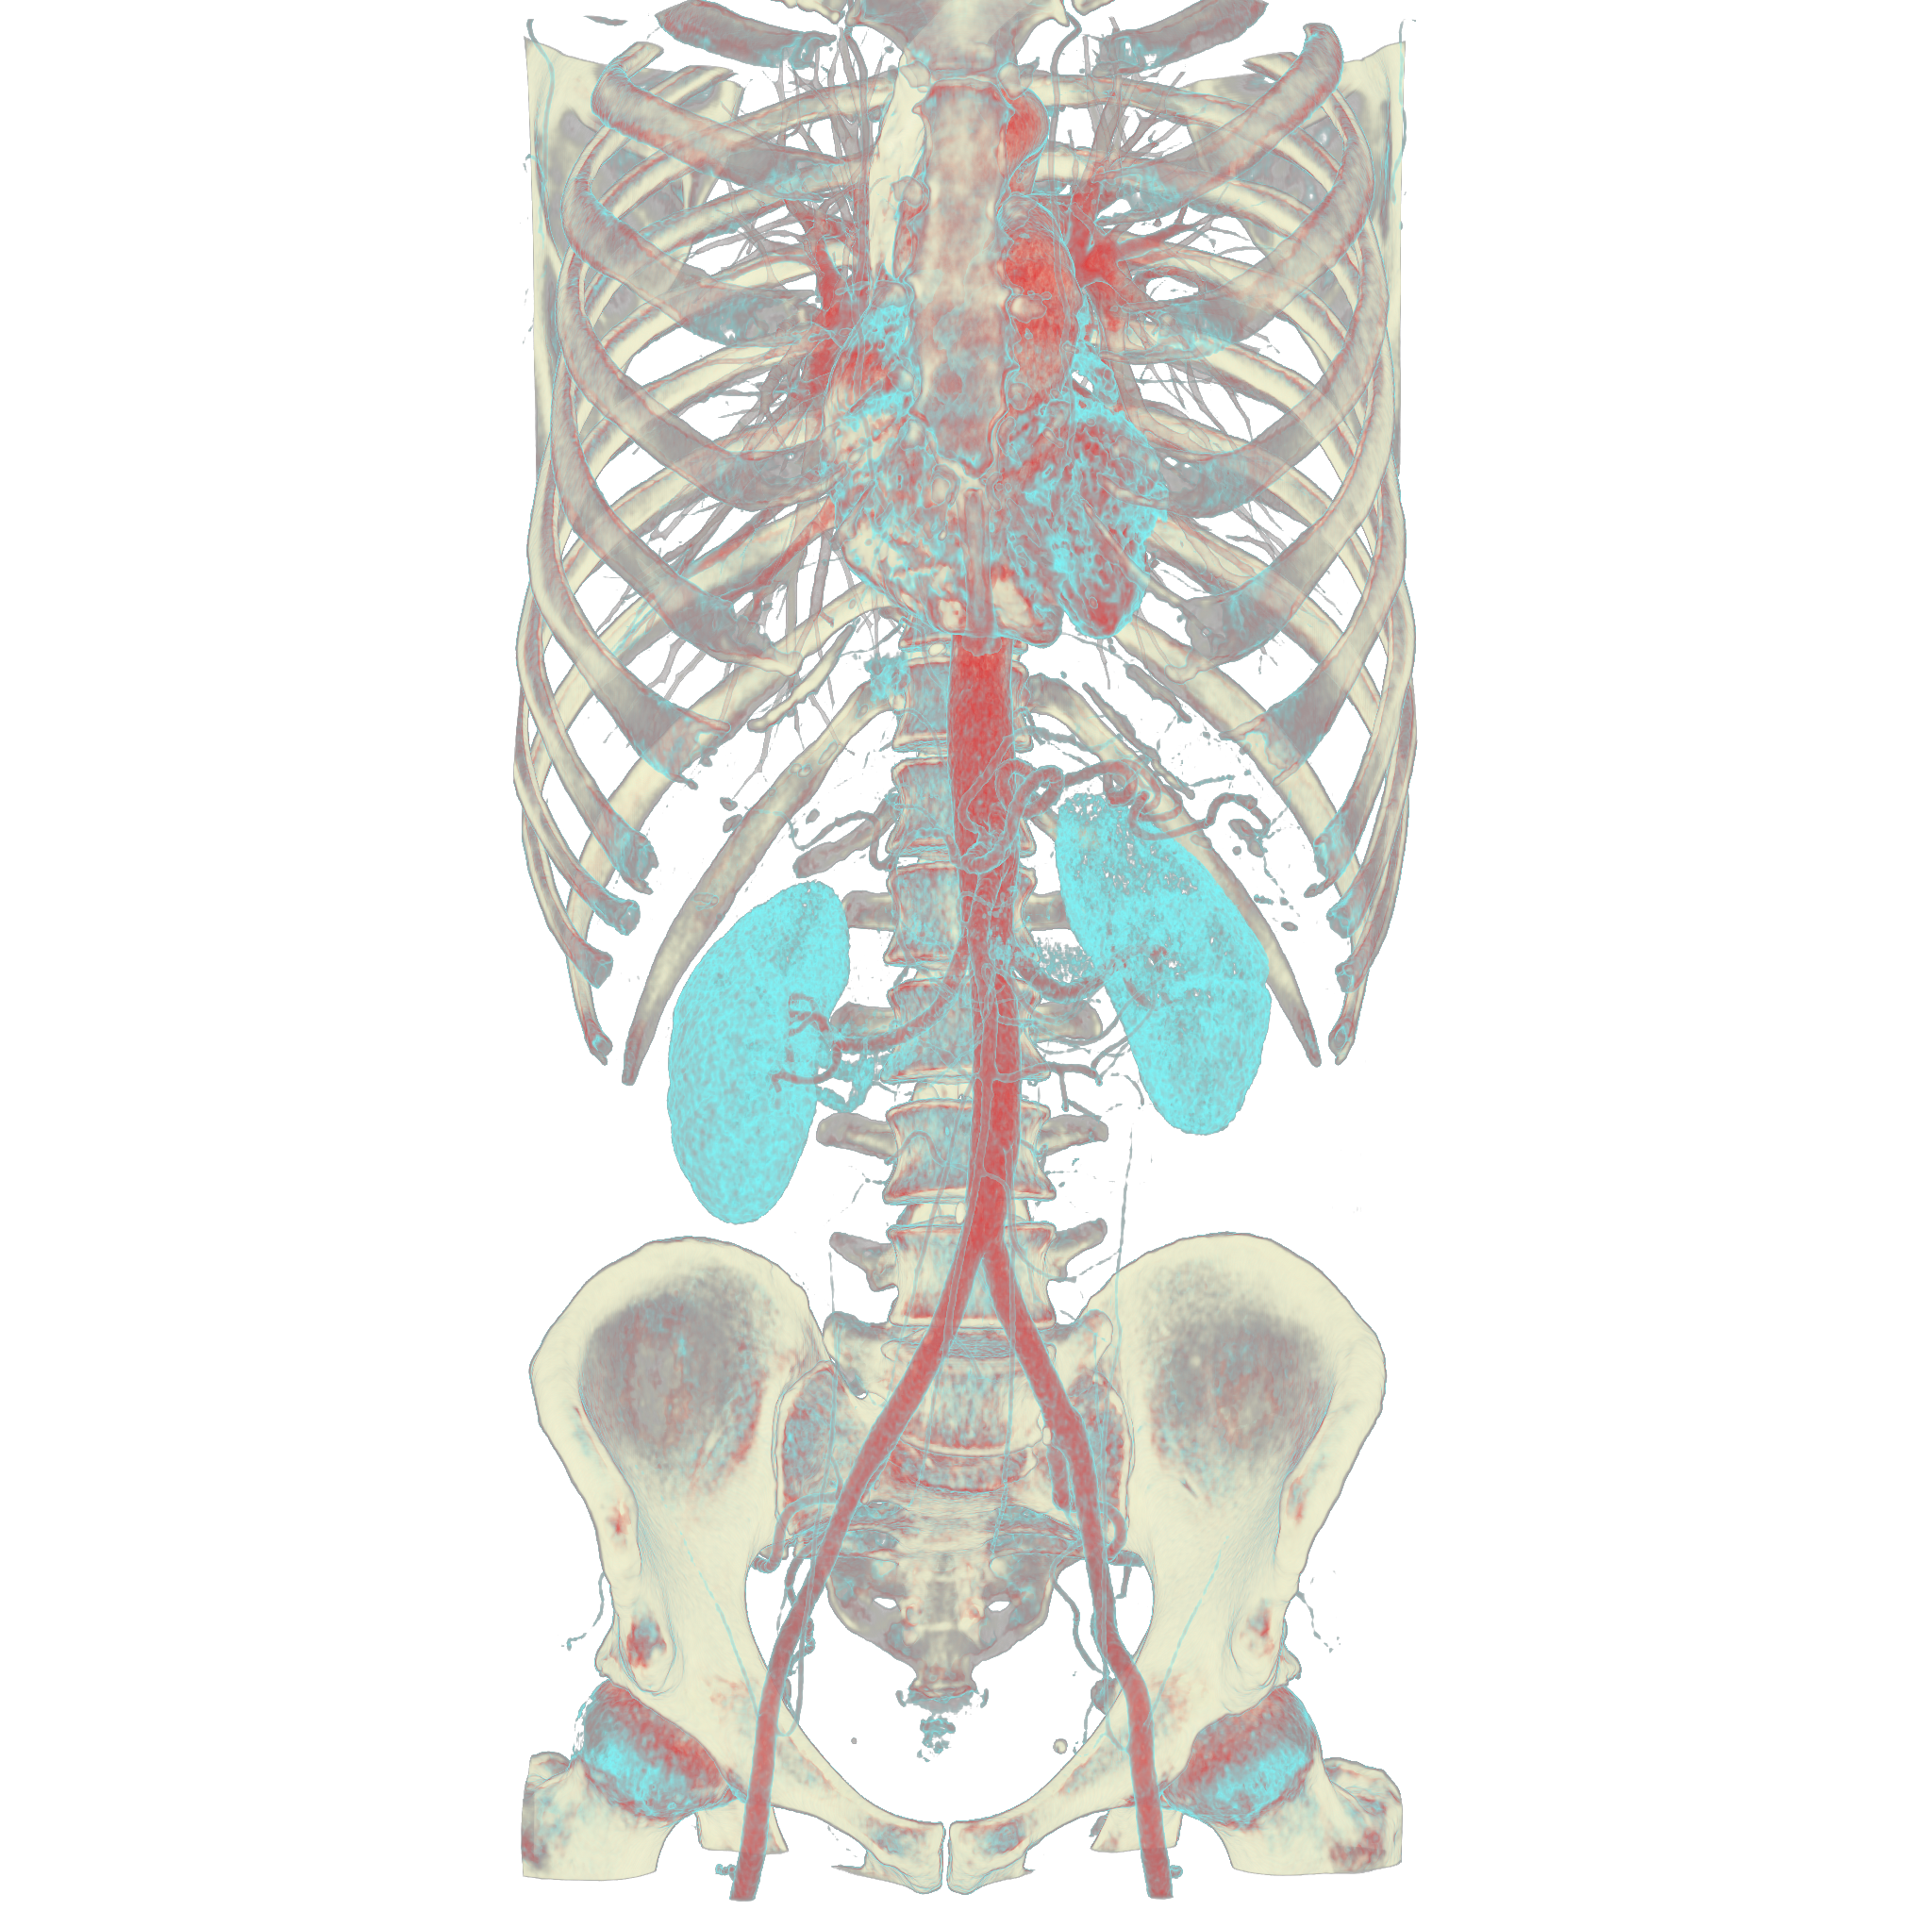
\includegraphics[width=\columnwidth]{colorimage}
    \caption{Color image}
    \label{fig:rendertotexturecolor}
  \end{subfigure}%
  \begin{subfigure}[b]{.5\columnwidth}
    \centering
    
\includegraphics[width=\columnwidth]{depthimage}
    \caption{Depth image}
    \label{fig:rendertotexturedepth}
  \end{subfigure}
  \caption{When~\texttt{RenderToImage} is enabled, the color and depth data of
    the final rendering is written to a texture object which can be used for
    further processing}
  \label{fig:rendertotexture}
\end{figure}

When the \texttt{RenderToImage} flag is enabled, the volume mapper switches
rendering to an OpenGL FrameBufferObject (FBO) and allows the user to obtain the
rendered pixel data via simple image retrieval calls. The mapper provides
methods to grab color and depth information either as individual textures or as
VTK's image data structure -~\texttt{vtkImageData}. The color data is simply the
pixel representation of the rendered volume whereas depth data consists of a
grayscale image depicting how deep each voxel is in the scene (as depicted
in~\Autoref{fig:rendertotexture}). When an application enables render to texture
mode, a framebuffer object is created, the vertex and fragment shader are
generated, color and depth buffers are cleared, and the color is set to white
with a value of zero alpha. The value of zero alpha is used so that applications
can safely ignore the transparent pixels and the color buffer is set to white
color because white represents the maximum depth, that is the depth of the far
plane. In the render to texture pass, the fragment shader writes to color and
depth target and to write the depth information it uses the depth of first
non-transparent voxel.

\subsection{Stochastic Jittering}
\label{jittering}
Because ray-casting effectively samples a discrete signal (voxel values along
the ray trajectory), the distance between sampling points heavily influences how
accurately the volume data is represented.  Due to well established limitations
described by the sampling theorem, low sampling rates may result in aliasing
effects often referred to as wood-grain artifacts as shown
in~\Autoref{fig:jittering_without} in the context of volume
rendering~\citep{engel_real-time_2006}. Reducing the distance between samples
neutralizes these artifacts but takes an important toll on performance.

The mapper supports stochastic jittering, which is an alternative technique to
counteract wood-grain artifacts by adding a random offset to the rays in the
viewing direction thereby breaking the coherence between neighboring fragments
which causes the aliased patterns become less apparent as shown
in~\Autoref{fig:jittering_with}.  Jittering is implemented by creating a random
noise texture (using~\texttt{vtkPerlinNoise}) and applying the offset to the
ray's starting point, thus has a much lower performance penalty than reducing
the sampling distance.

\begin{figure}[htb]
\centering
  \begin{subfigure}[b]{.5\columnwidth}
    \centering
    \includegraphics[width=\textwidth]{cactus_holland_woodgrain}
    \caption{Wood-grain artifacts.}
    \label{fig:jittering_without}
  \end{subfigure}%
  \begin{subfigure}[b]{.5\columnwidth}
    \centering
    \includegraphics[width=\textwidth]{cactus_holland_jittering}
    \caption{Jittering enabled.}
    \label{fig:jittering_with}
  \end{subfigure}
  \caption{Cactus sample scanned at Beamline 8.3.2, Advanced Light Source,
  Lawrence Berkeley National Laboratory. A coarse ray-sampling distance causes
  wood-grain artifacts to appear (a). Same data and sampling distance with
  stochastic jittering enabled to mitigate the artifacts (b).}
  \label{fig:jittering}
\end{figure}

\subsection{Clipping}
\label{clipping}
A set of infinite planes can be defined to clip the volume to reveal inner
detail, as shown in Figure 4.  The visibility of each sample along the ray
is determined by computing the sample's distance to each plane and testing
for it being in front or behind.

The current implementation iterates through each of the planes before entering
the ray marching loop in order to early-discard rays which fall in any of the
following criteria:

\begin{enumerate}
\item Entering the volume on the clipped side and exiting before ever
  intersecting the plane (the ray only traverses clipped space).
\item Intersecting overlapping geometry before the plane (z-buffer compositing).
\end{enumerate}

\subsection{Cropping}
\label{cropping}
Cropping refers to the 27 regions defined by pairs of
planes along each volume coordinate axis and can be independently turned
on (visible) or off (invisible) to produce a variety of different cropping
effects%, as shown in ~\Autoref{fig:cropping}.
Cropping is implemented by determining the cropping region of each sample
location along the ray and including only those samples that fall within
a visible region.

% \begin{figure}[htb]
%   \centering
%   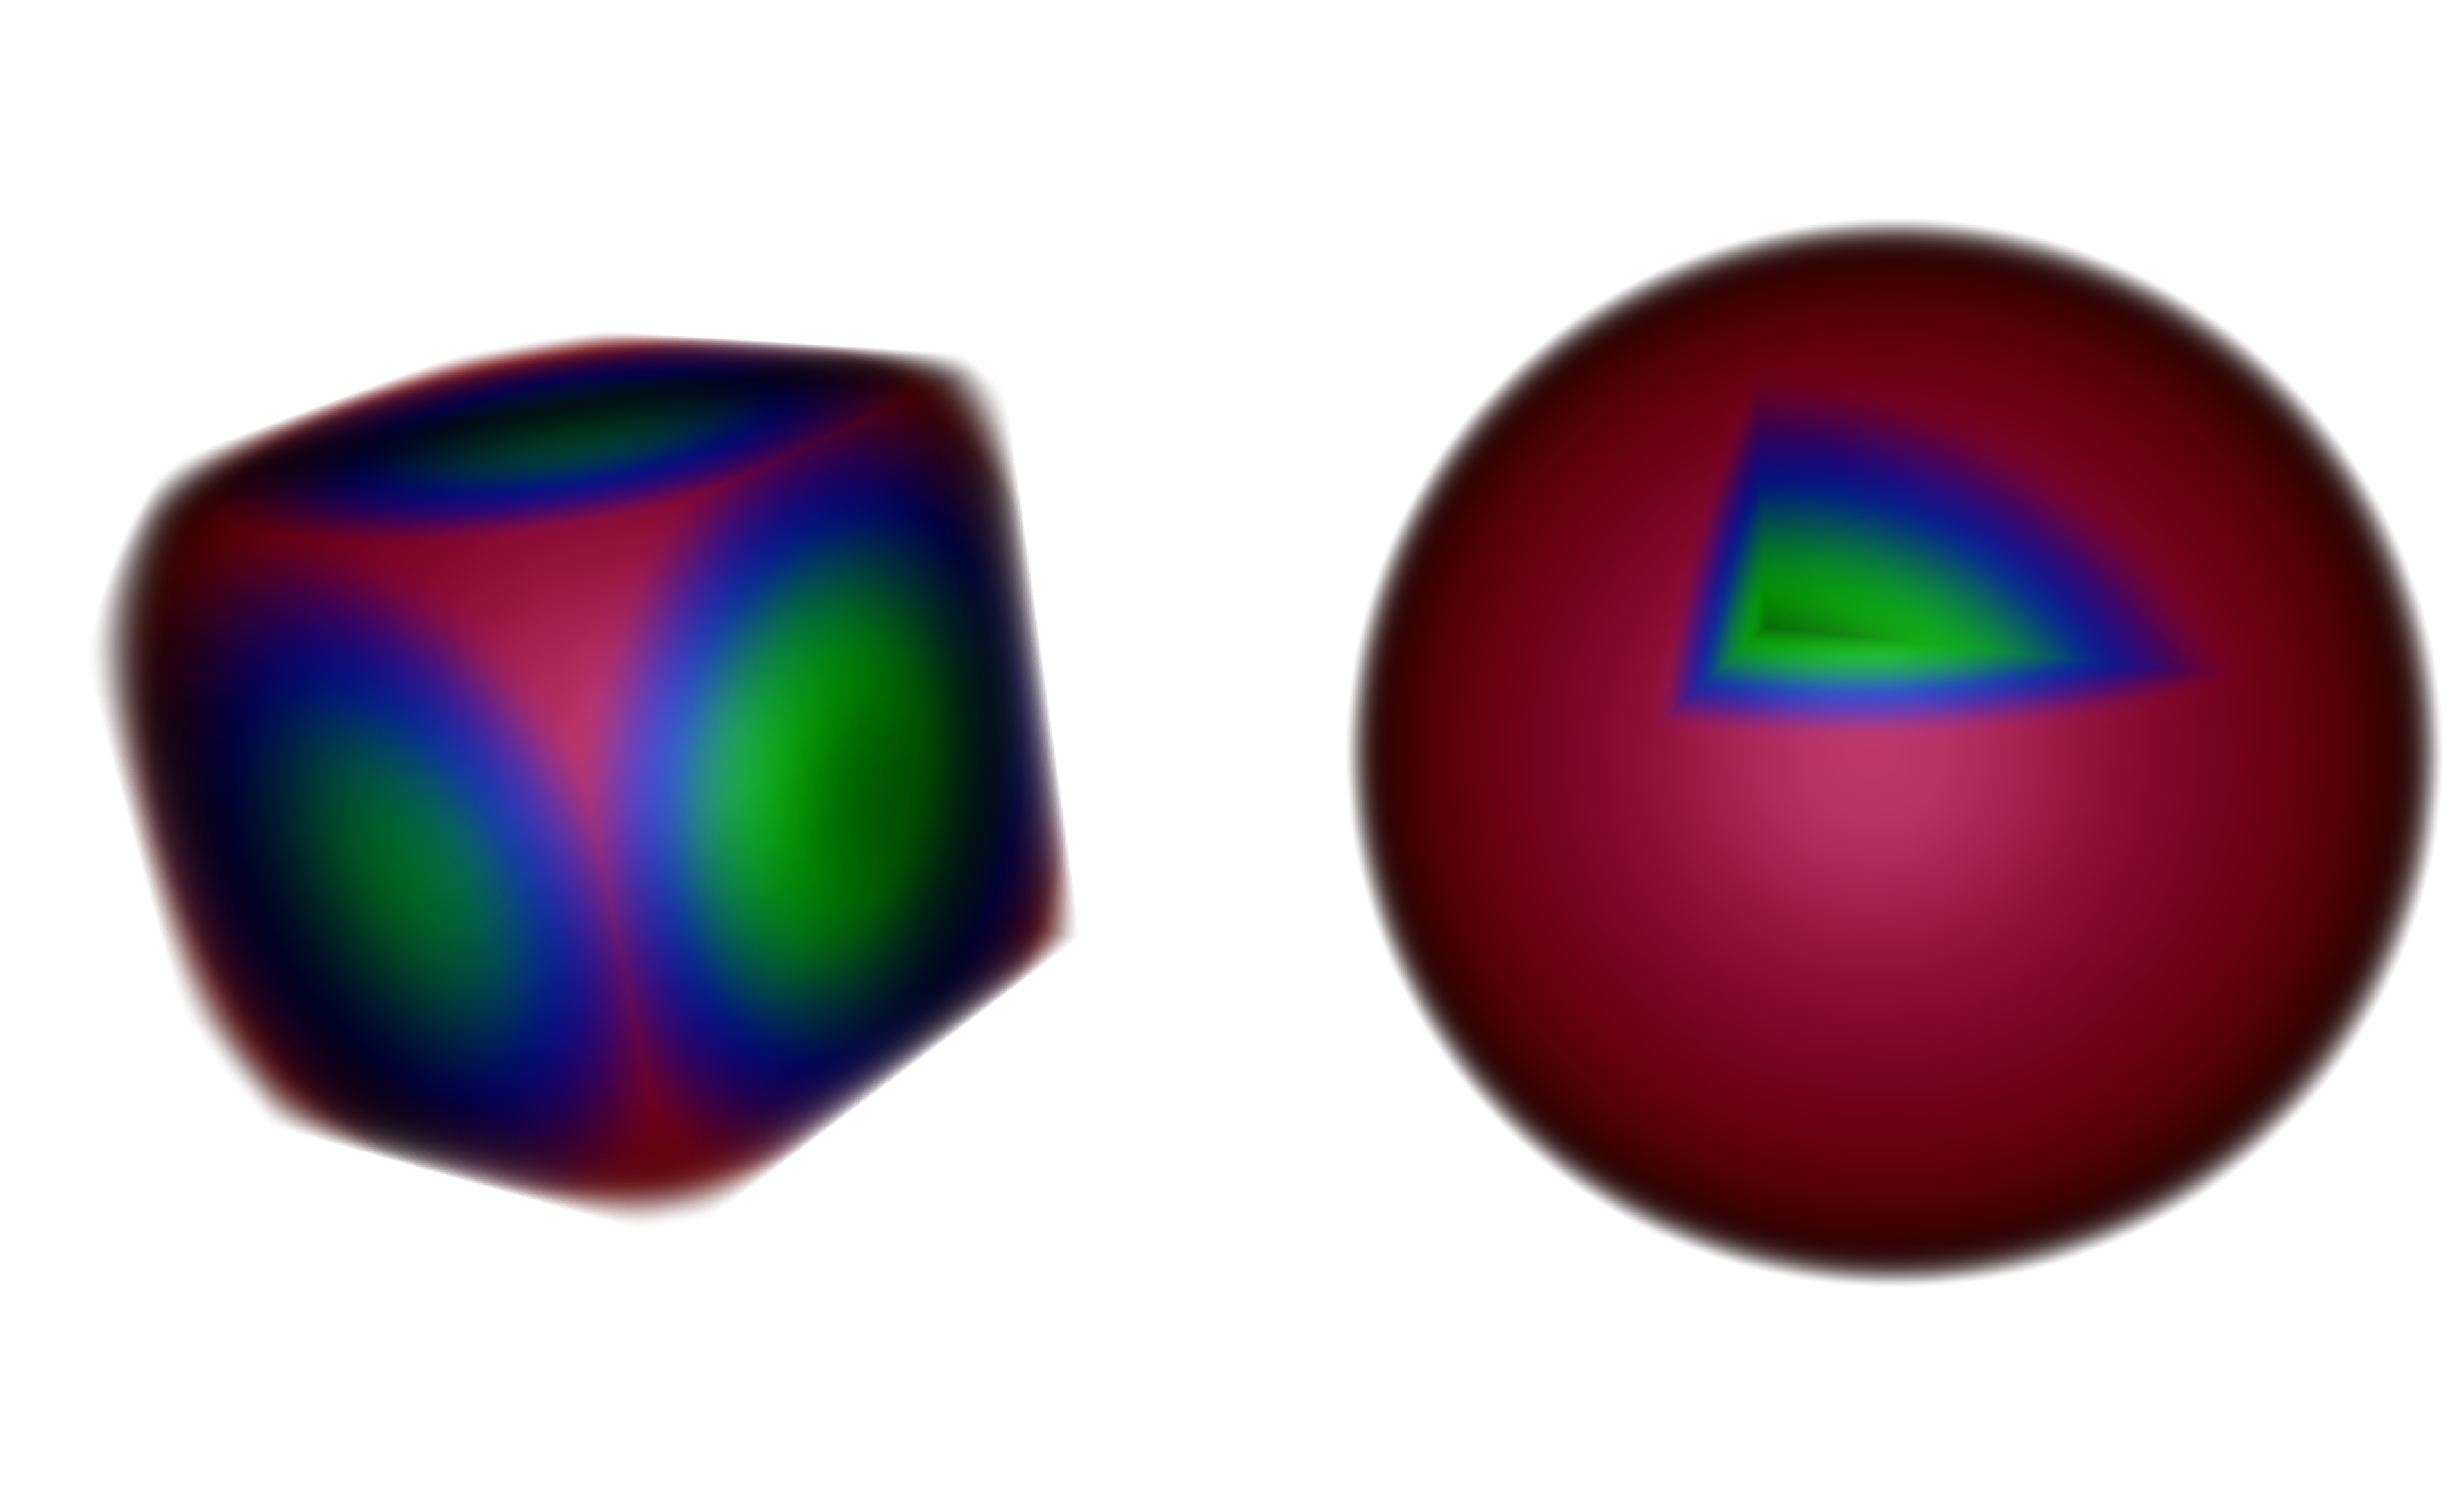
\includegraphics[width=2.5in]{SphereCropping.png}
%   \caption{A sphere is cropped using two different configurations of cropping regions.}
%   \label{fig:cropping}
% \end{figure}

\subsection{Broad Support of Data Types}
\label{data-types}
The mapper supports most signed and unsigned data types such as short, int,
float and double as well as the two most common data abstractions in VTK,
cell and point data.  Bias and scale factors are pre-computed and passed into
the fragment shader to normalize the data values for correct look-up table
mapping.

\begin{figure}[htb]
  \centering
  \begin{subfigure}[b]{\columnwidth}
    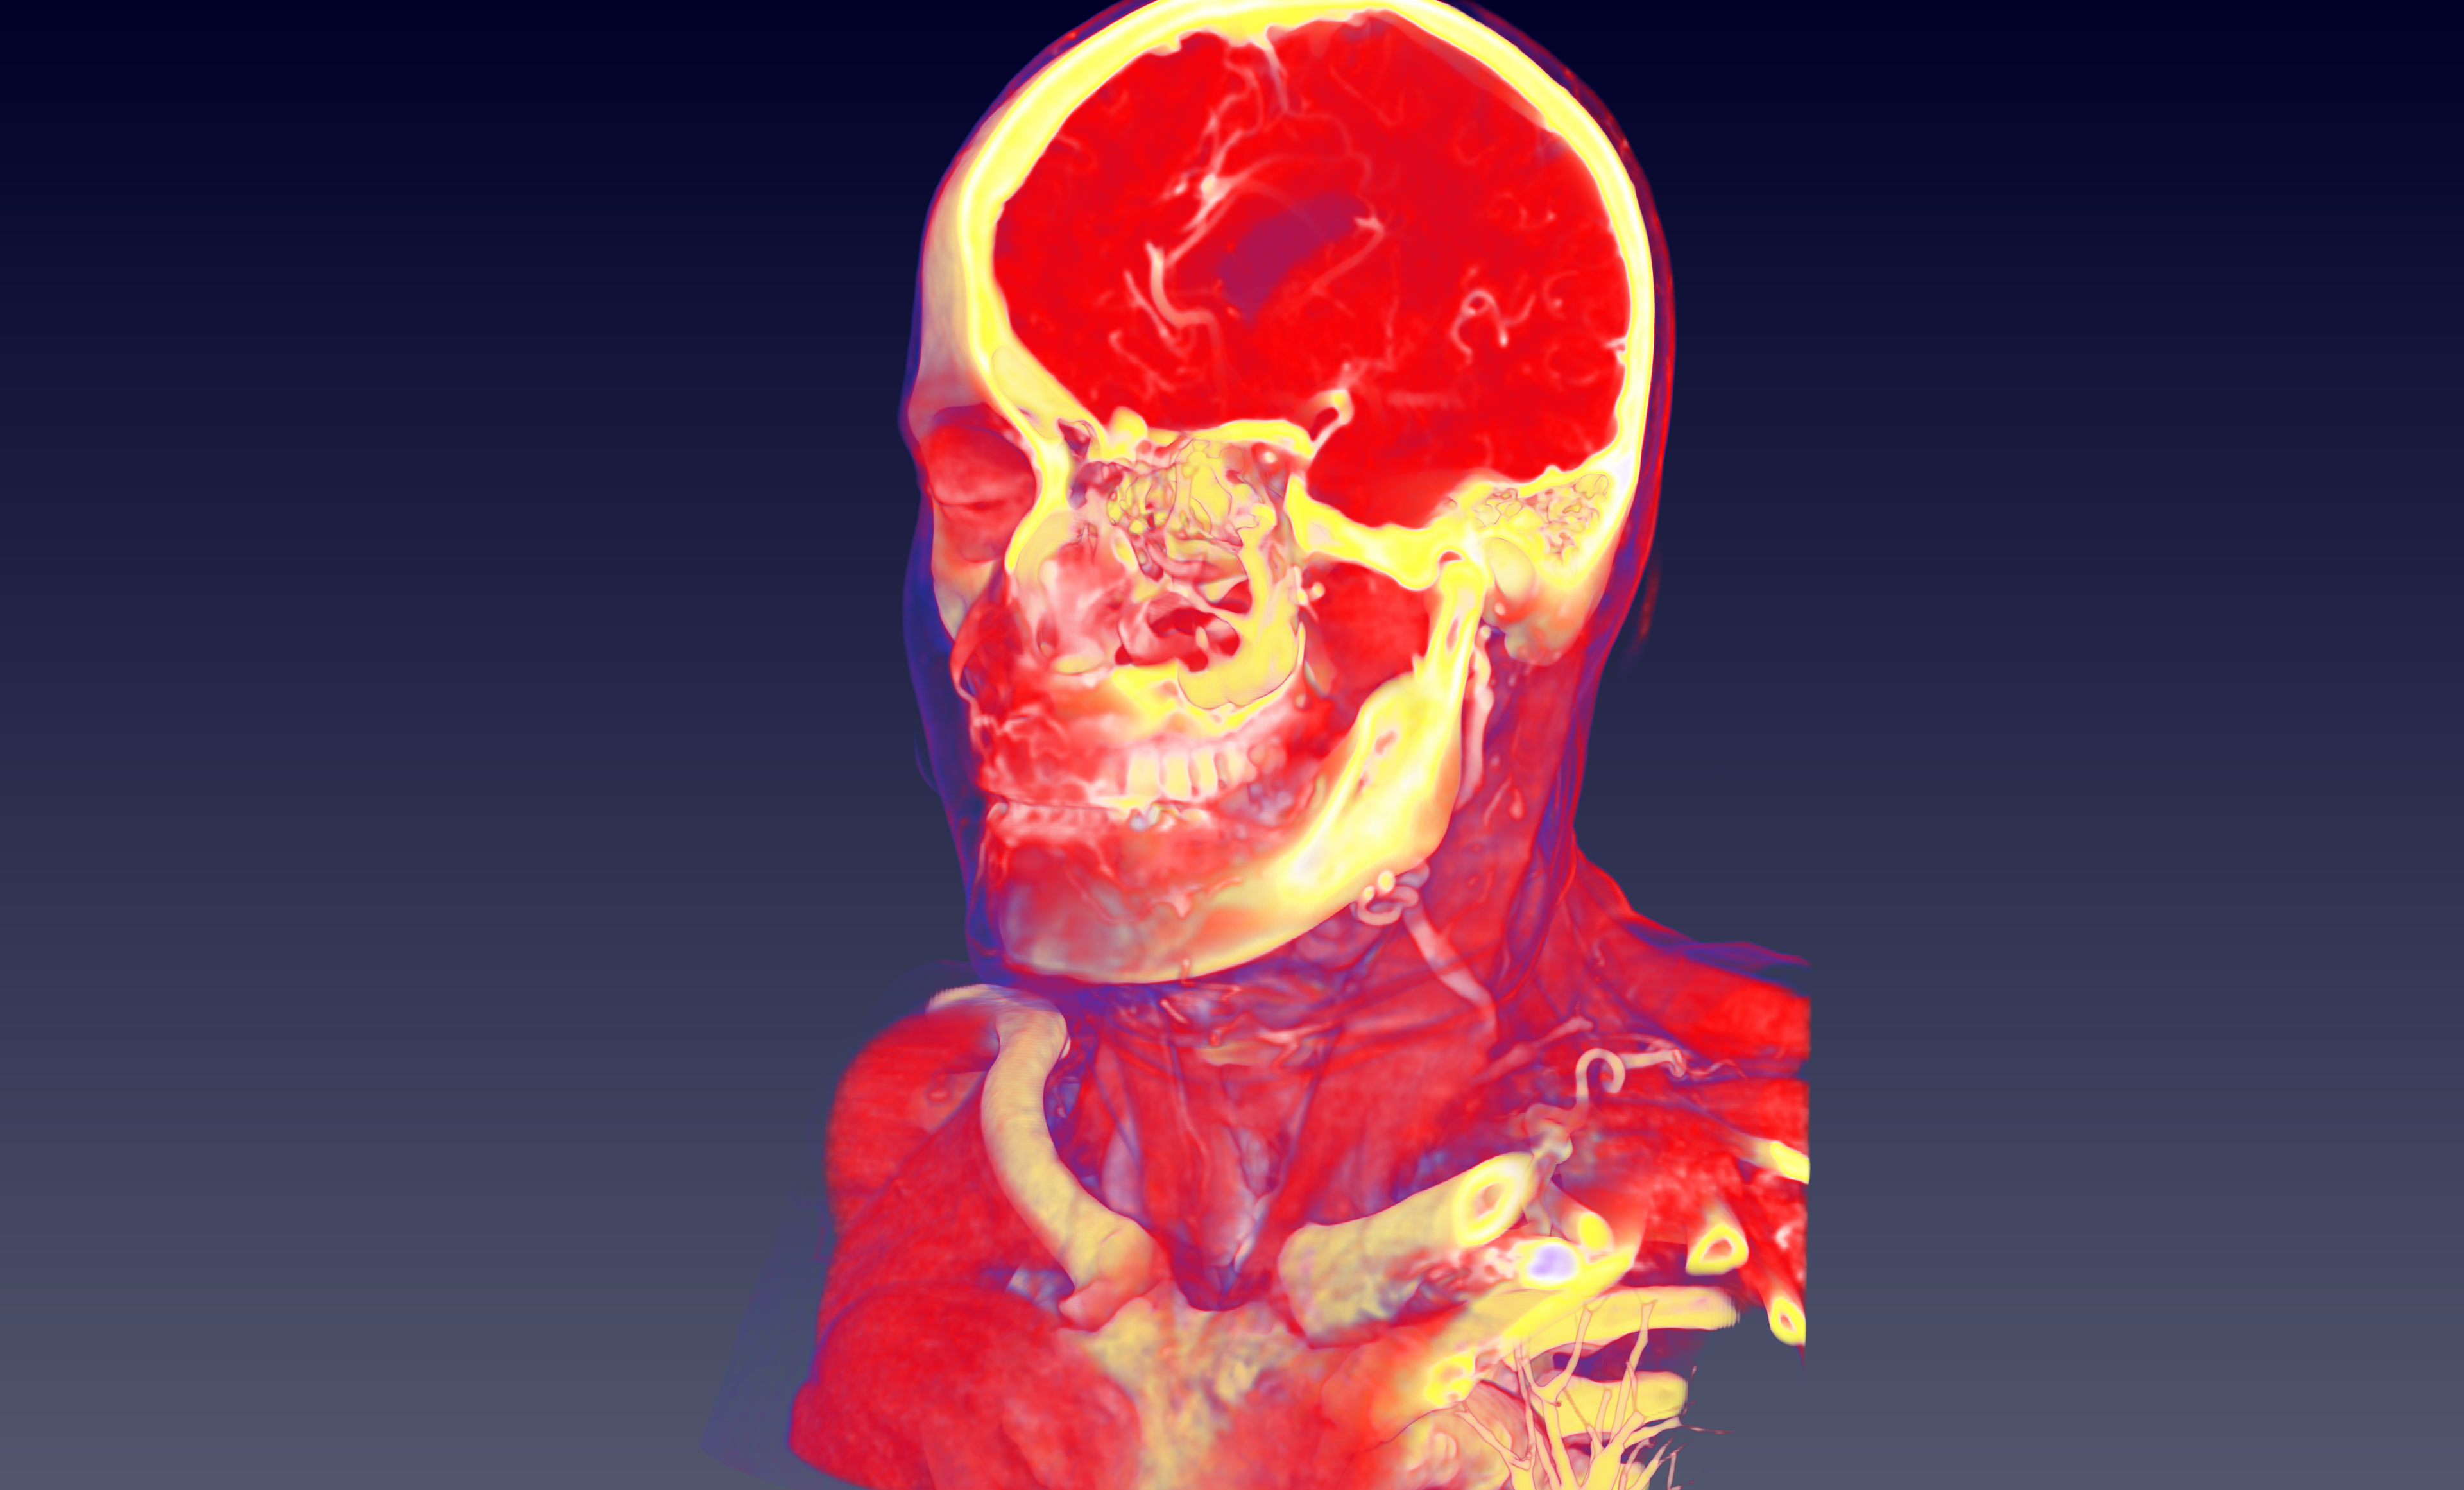
\includegraphics[width=\textwidth]{HeadClippingOblique}
    \caption{Clipping using an oblique clipping plane}
    \label{fig:clipoblique}
  \end{subfigure}
  \begin{subfigure}[b]{.5\columnwidth}
    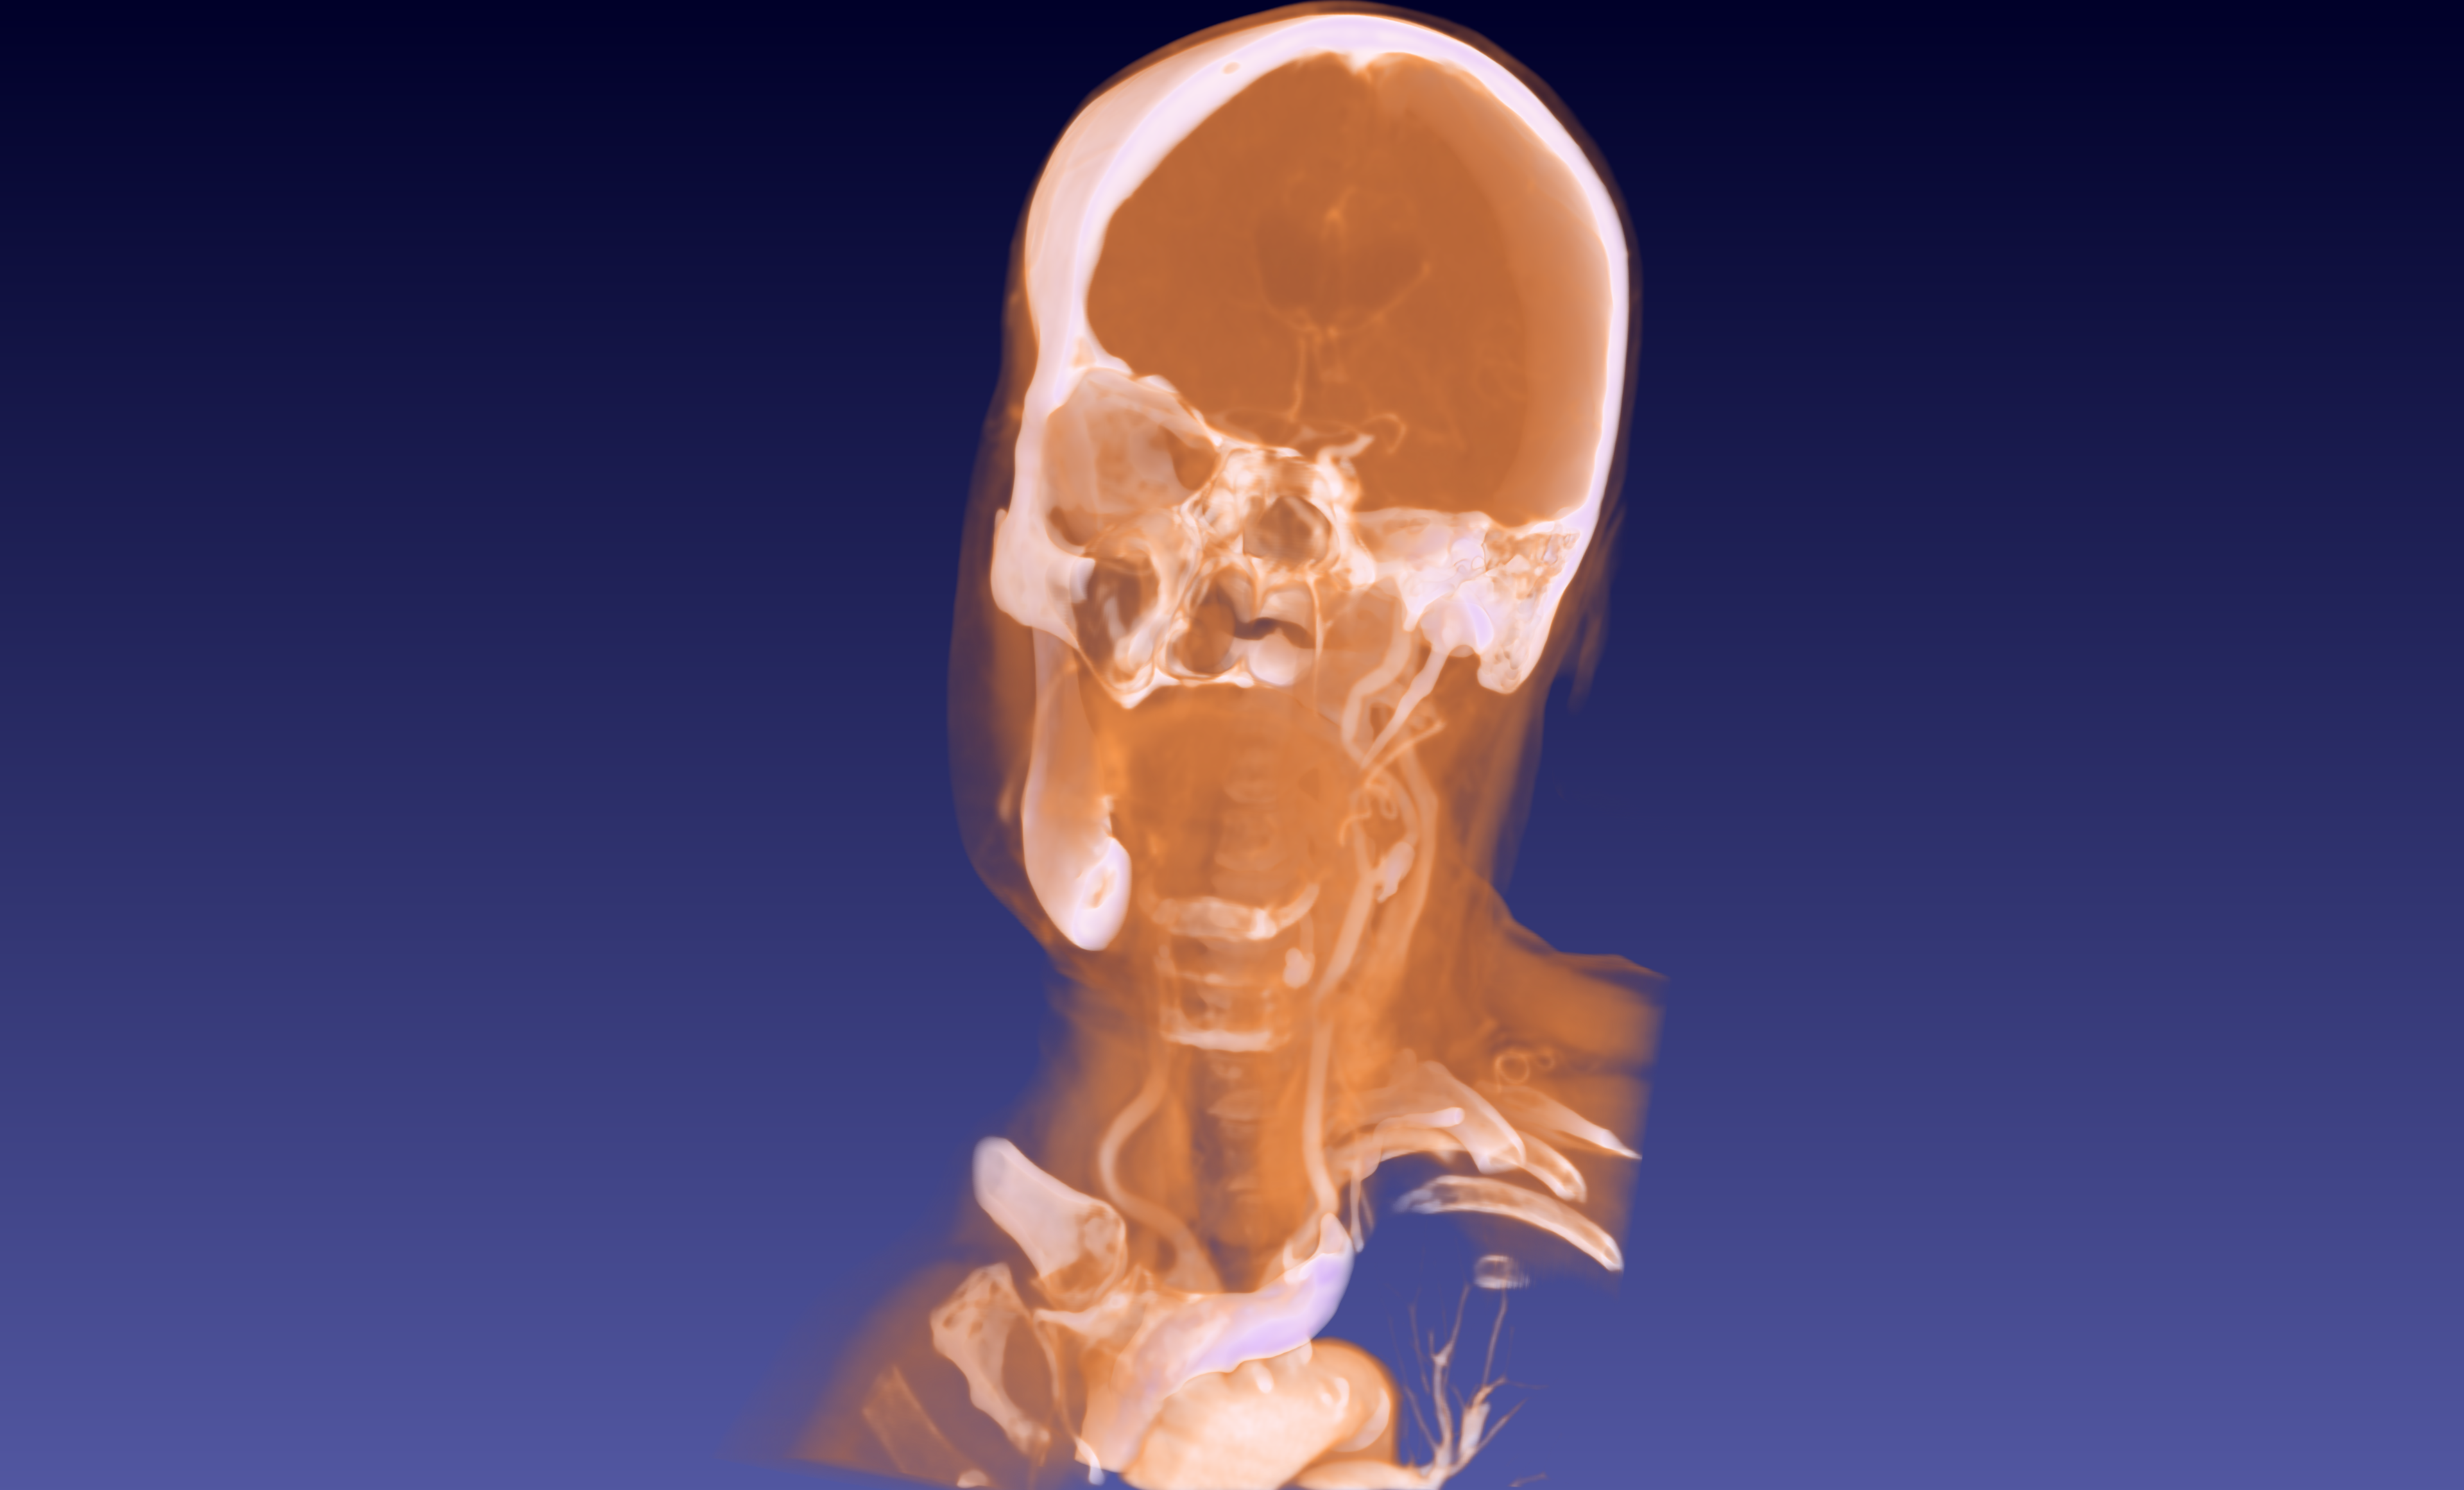
\includegraphics[width=\textwidth]{HeadClippingSlabNoShading}
    \caption{Without shading}
    \label{fig:clipnoshading}
  \end{subfigure}%
  \begin{subfigure}[b]{.5\columnwidth}
    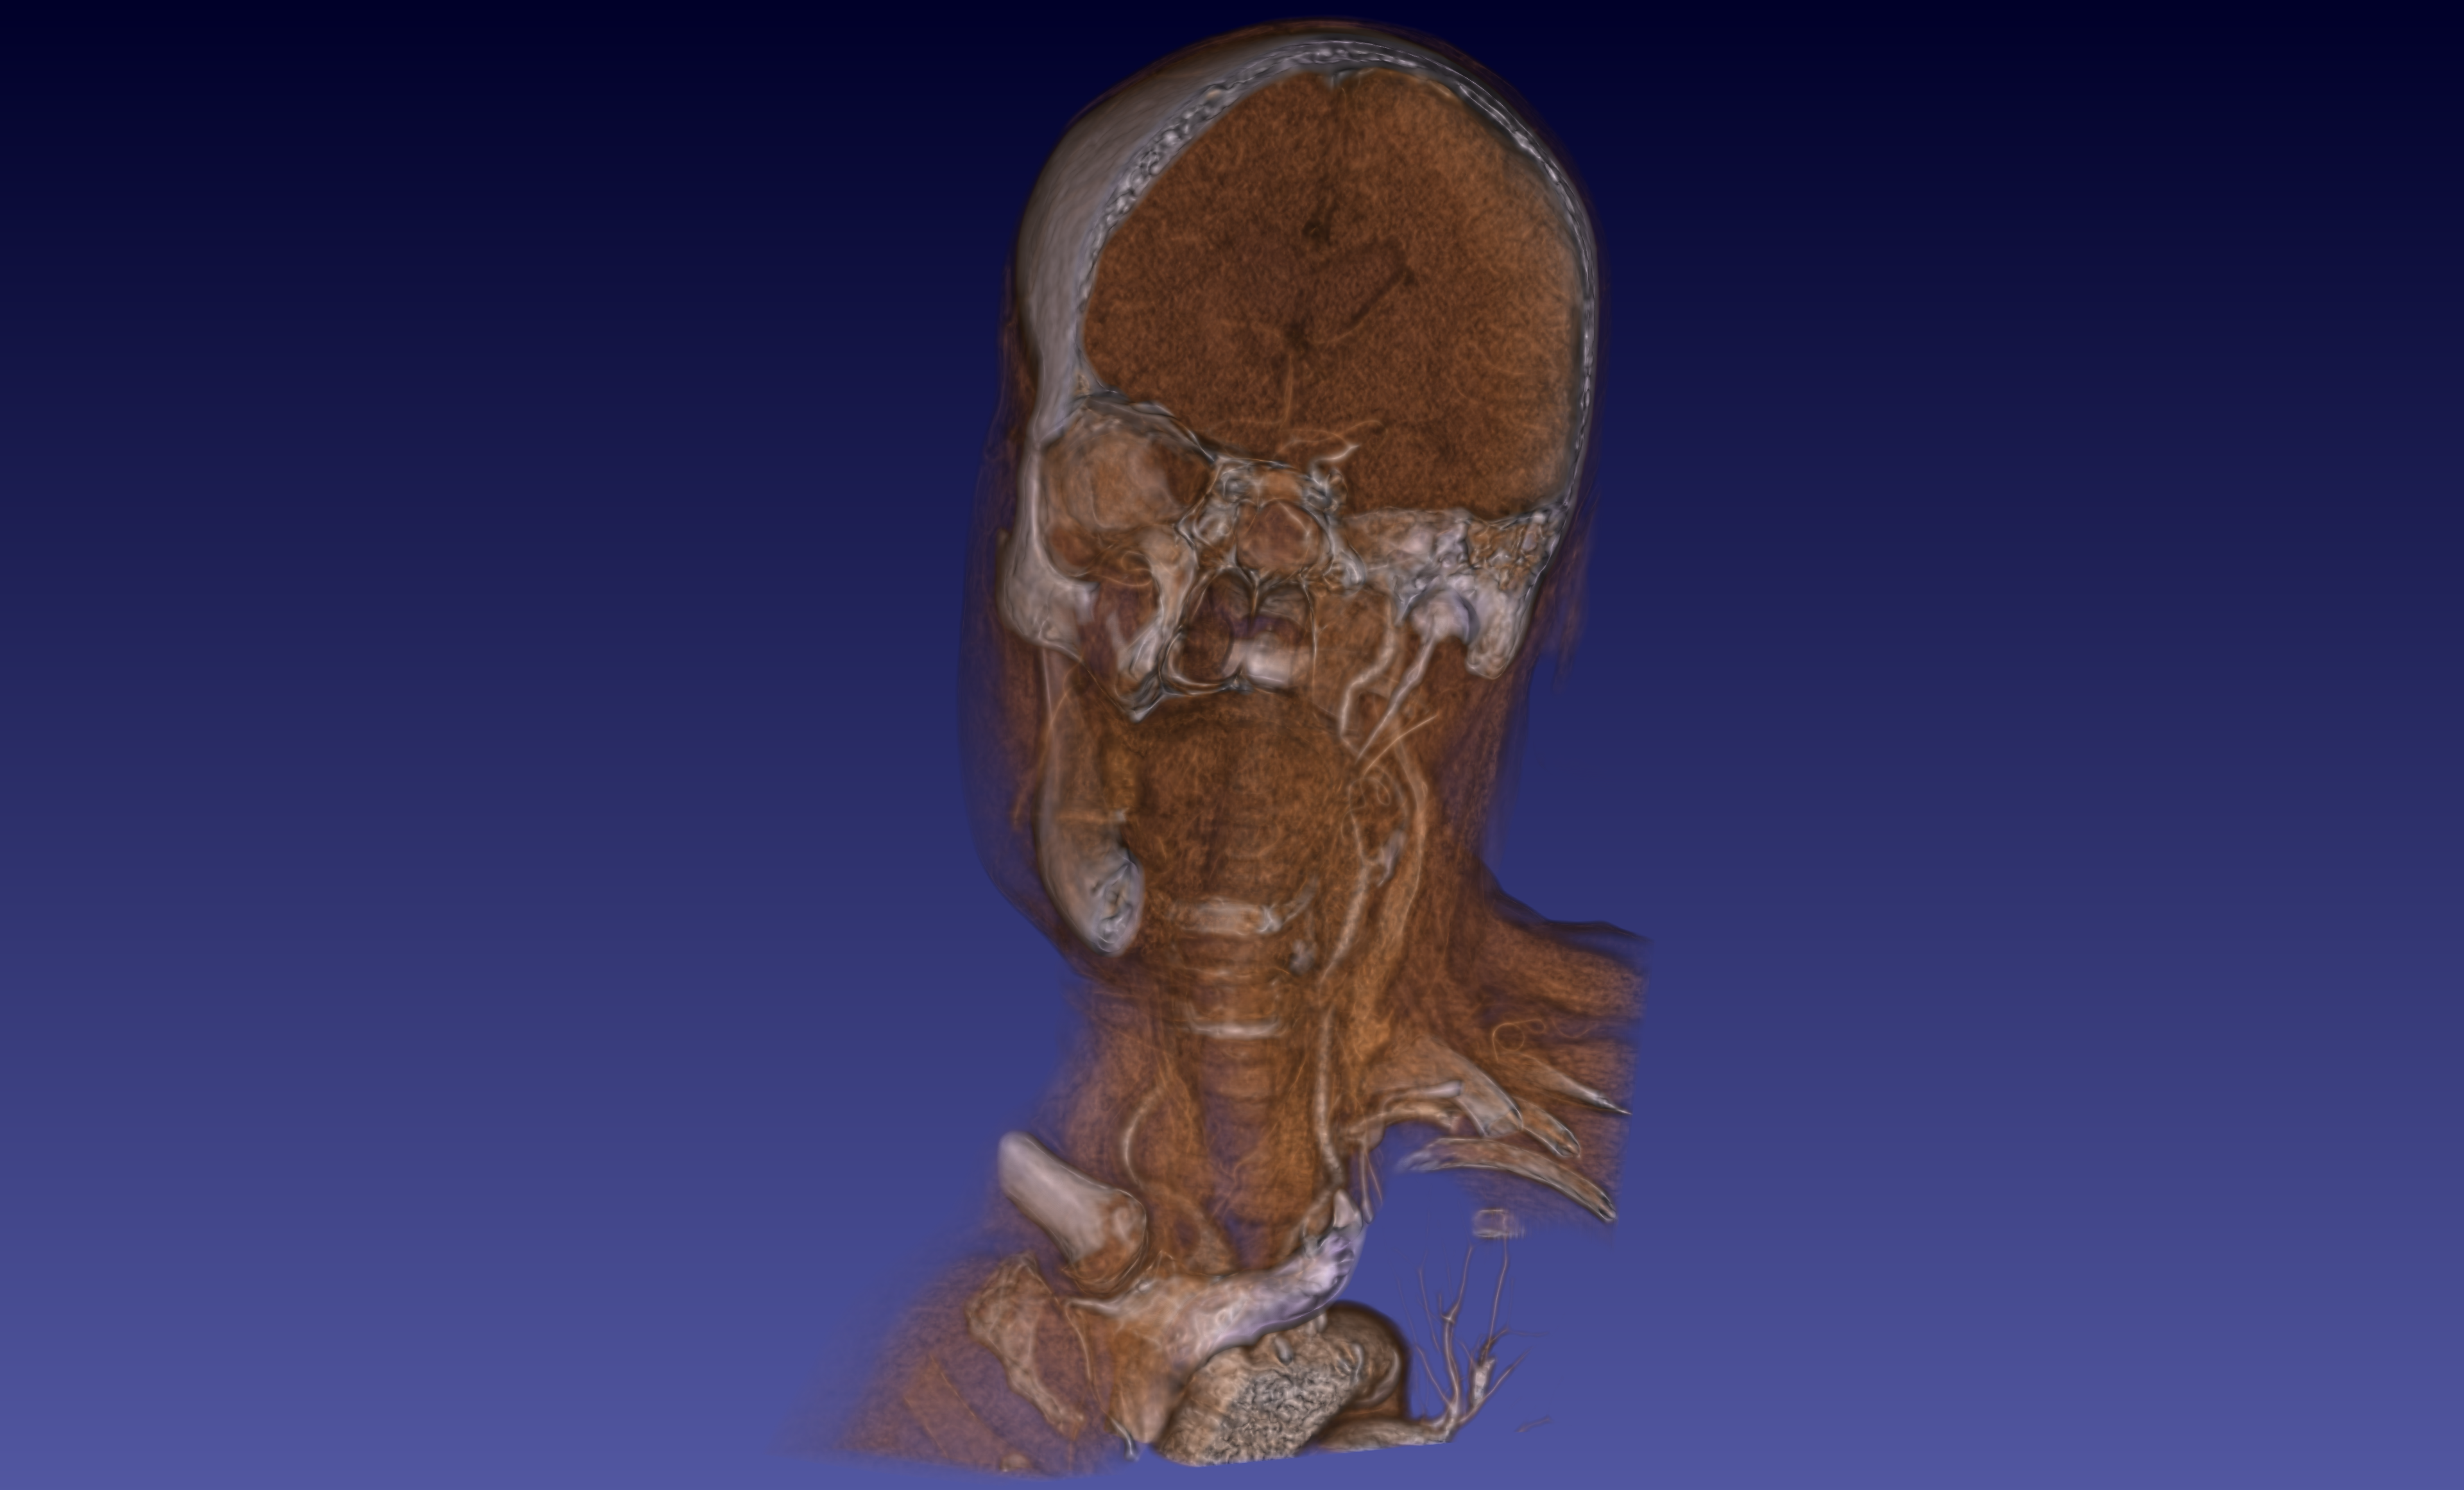
\includegraphics[width=\textwidth]{HeadClippingSlabShading}
    \caption{With shading}
    \label{fig:clipshading}
  \end{subfigure}
  \caption{Clipping planes with~\texttt{vtkGPUVolumeRayCastMapper}}
  \label{fig:clipping}
\end{figure}

\subsection{Blending Modes}
\label{blending-modes}
The mapper supports composite blending, minimum intensity projection, maximum
intensity projection, additive intensity and average intensity blending.  These
blending modes are useful for the variety of use case found in medical
computing.  The most common one which is also the default is the composite
blending mode.  See~\Autoref{fig:blendingmodes} for an example of the different
blend modes on the same data.

\begin{figure}[htb]
  \centering%
  \begin{subfigure}{.5\columnwidth}
    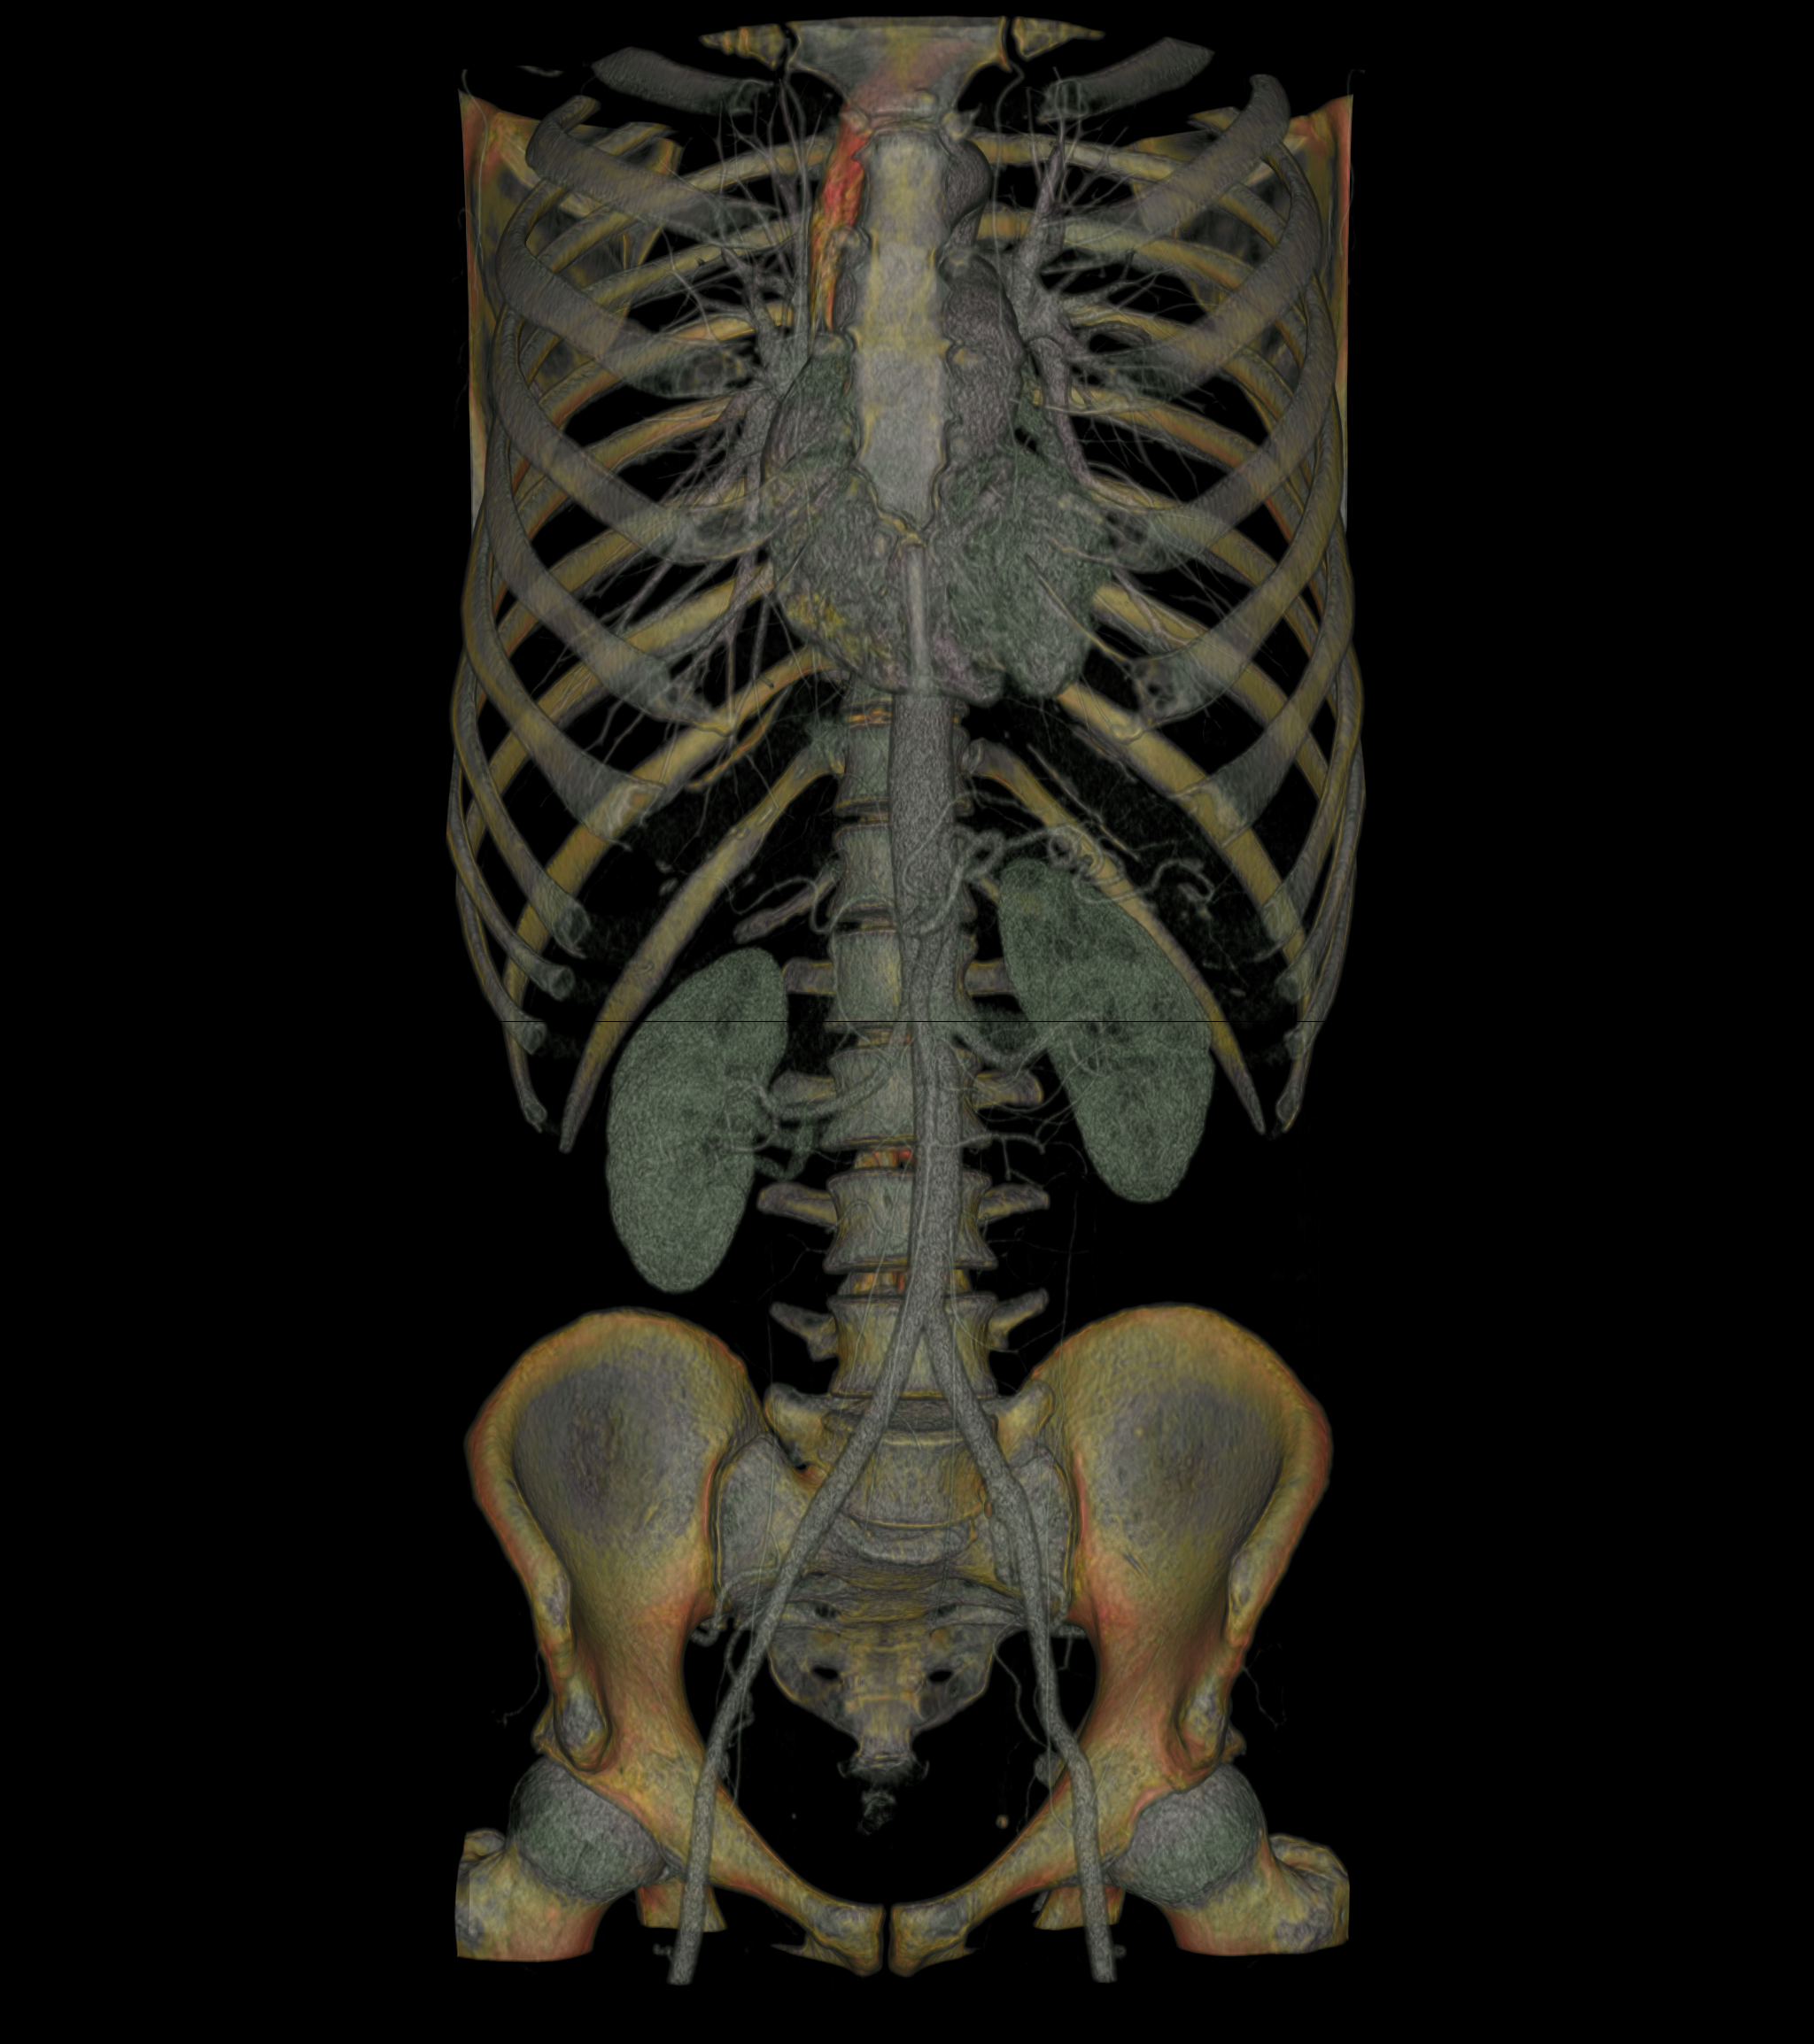
\includegraphics[width=\columnwidth]{TorsoBlendingComposite}
    \caption{Composite}
    \label{fig:blendcomposite}
  \end{subfigure}%
  \begin{subfigure}{.5\columnwidth}
    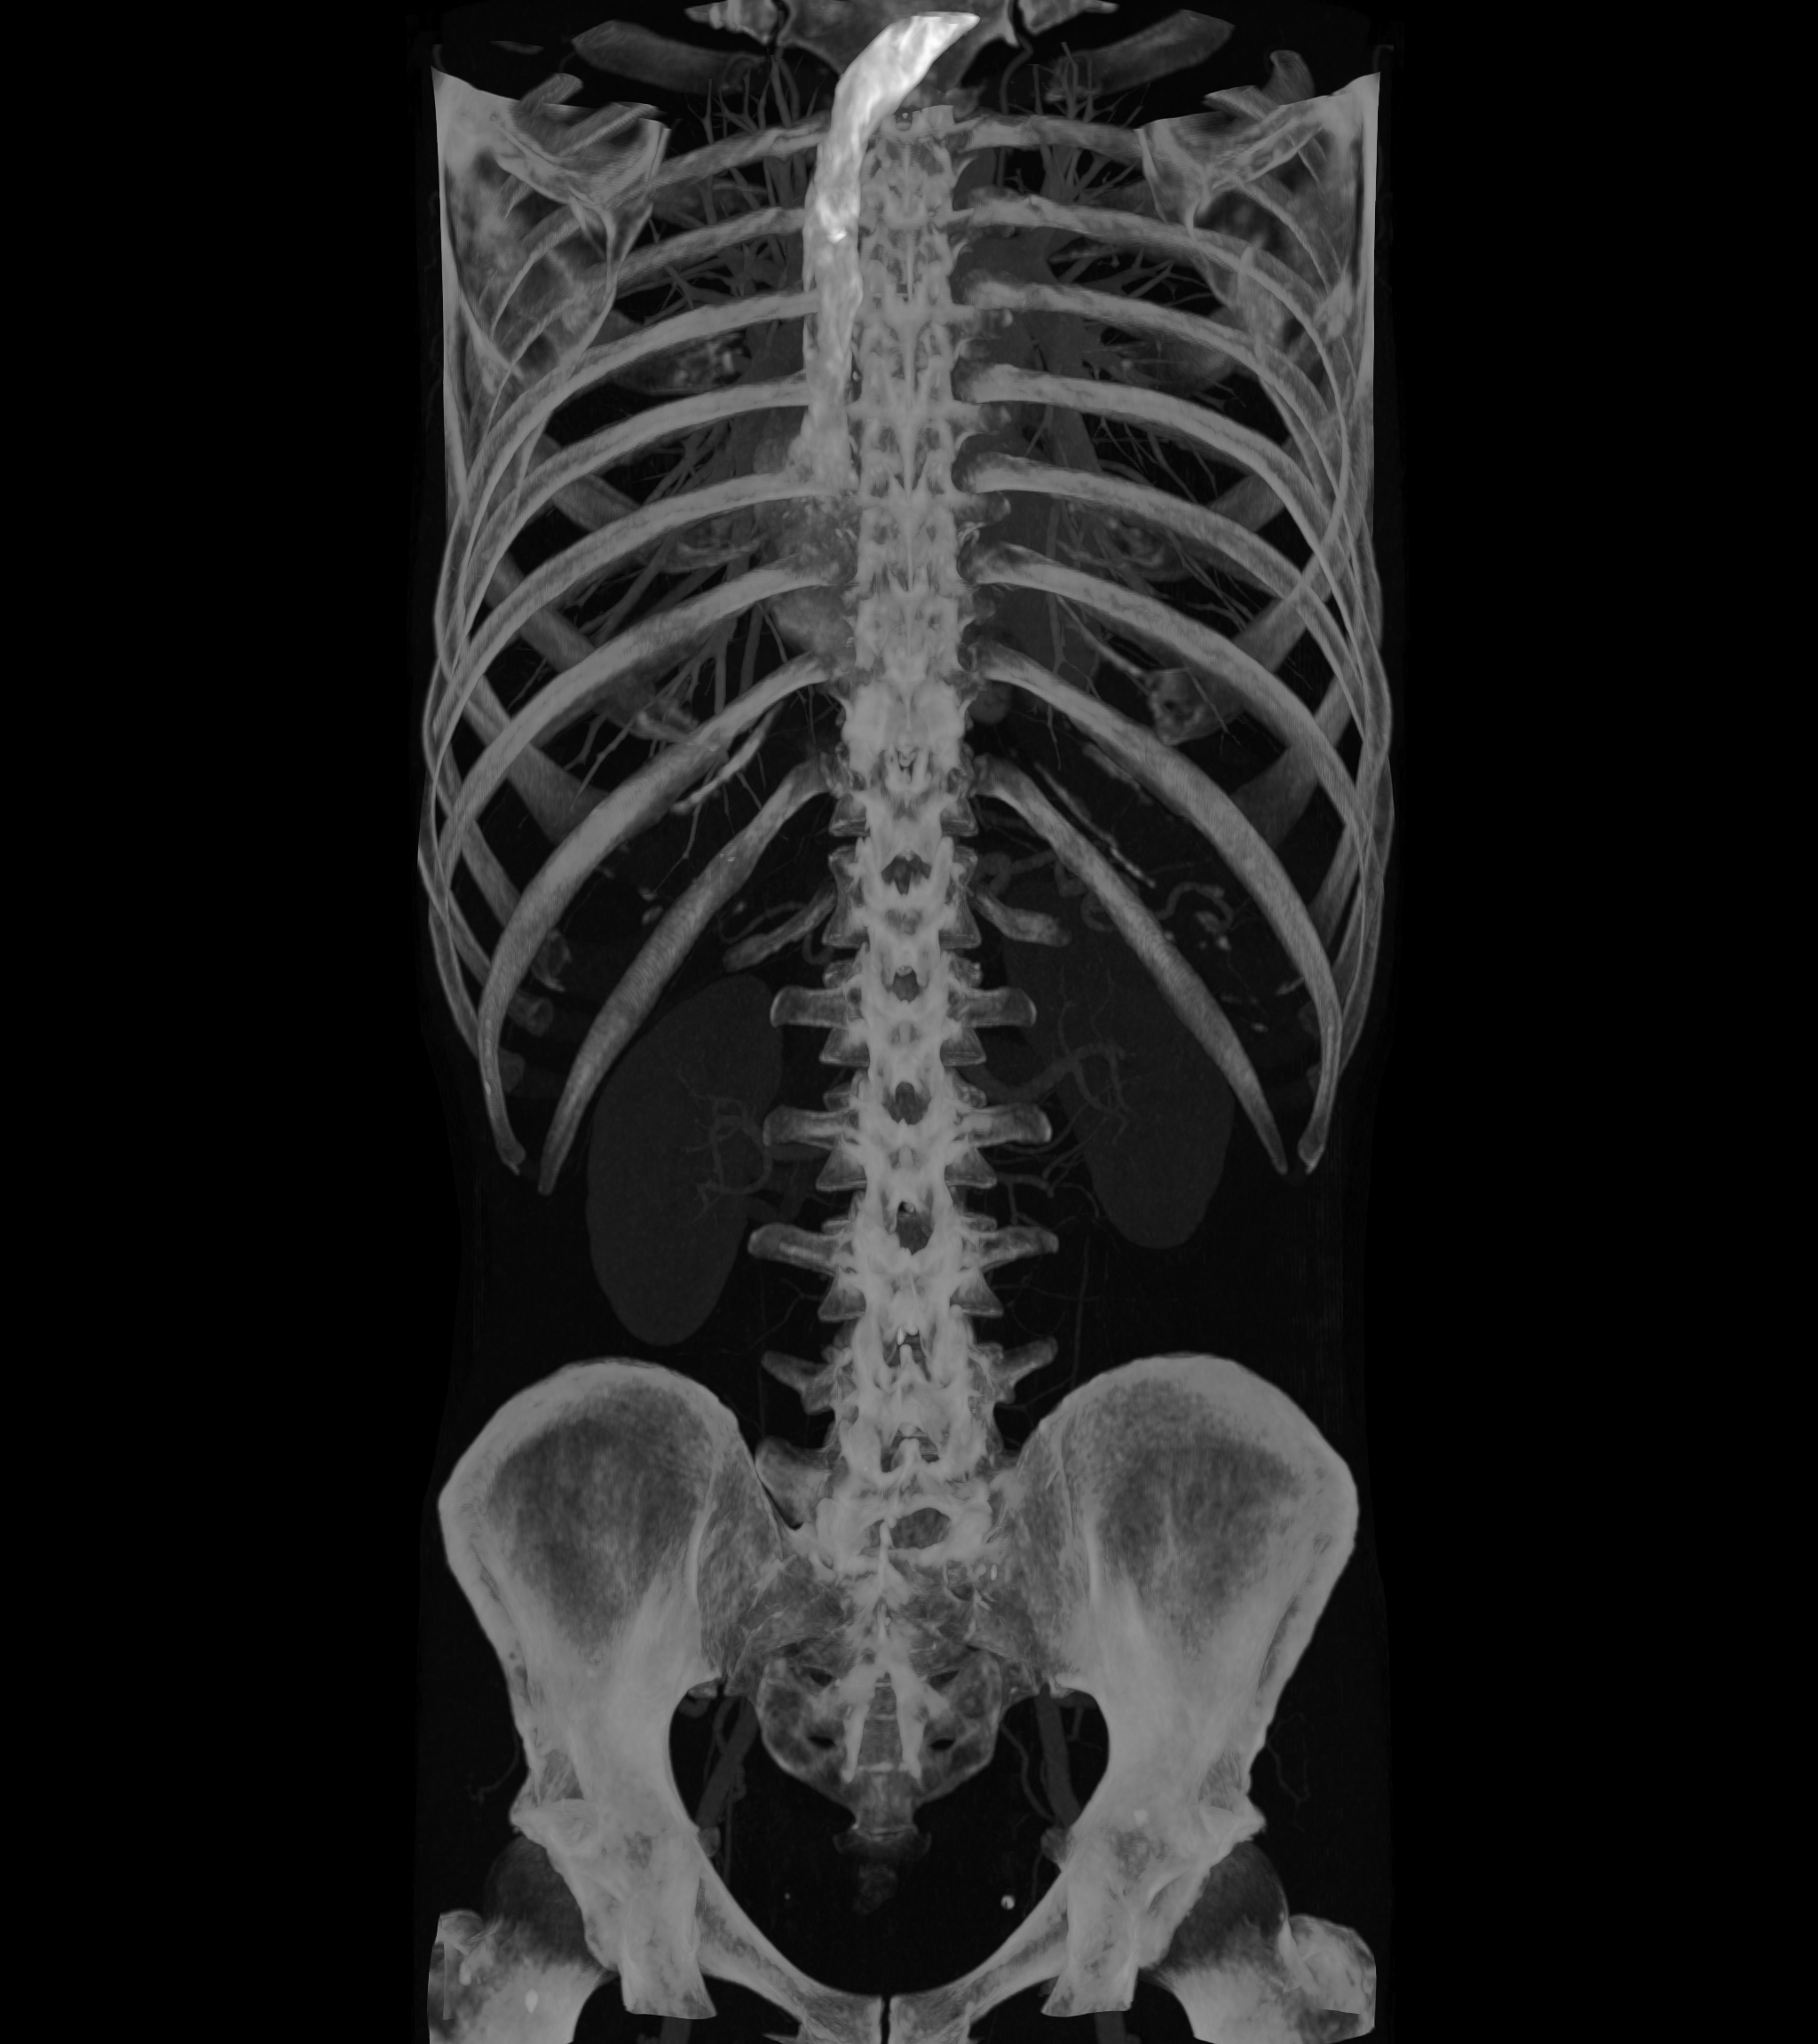
\includegraphics[width=\columnwidth]{TorsoBlendingMIP}
    \caption{Maximum Intensity}
    \label{fig:blendmax}
  \end{subfigure}
  \begin{subfigure}{.5\columnwidth}
    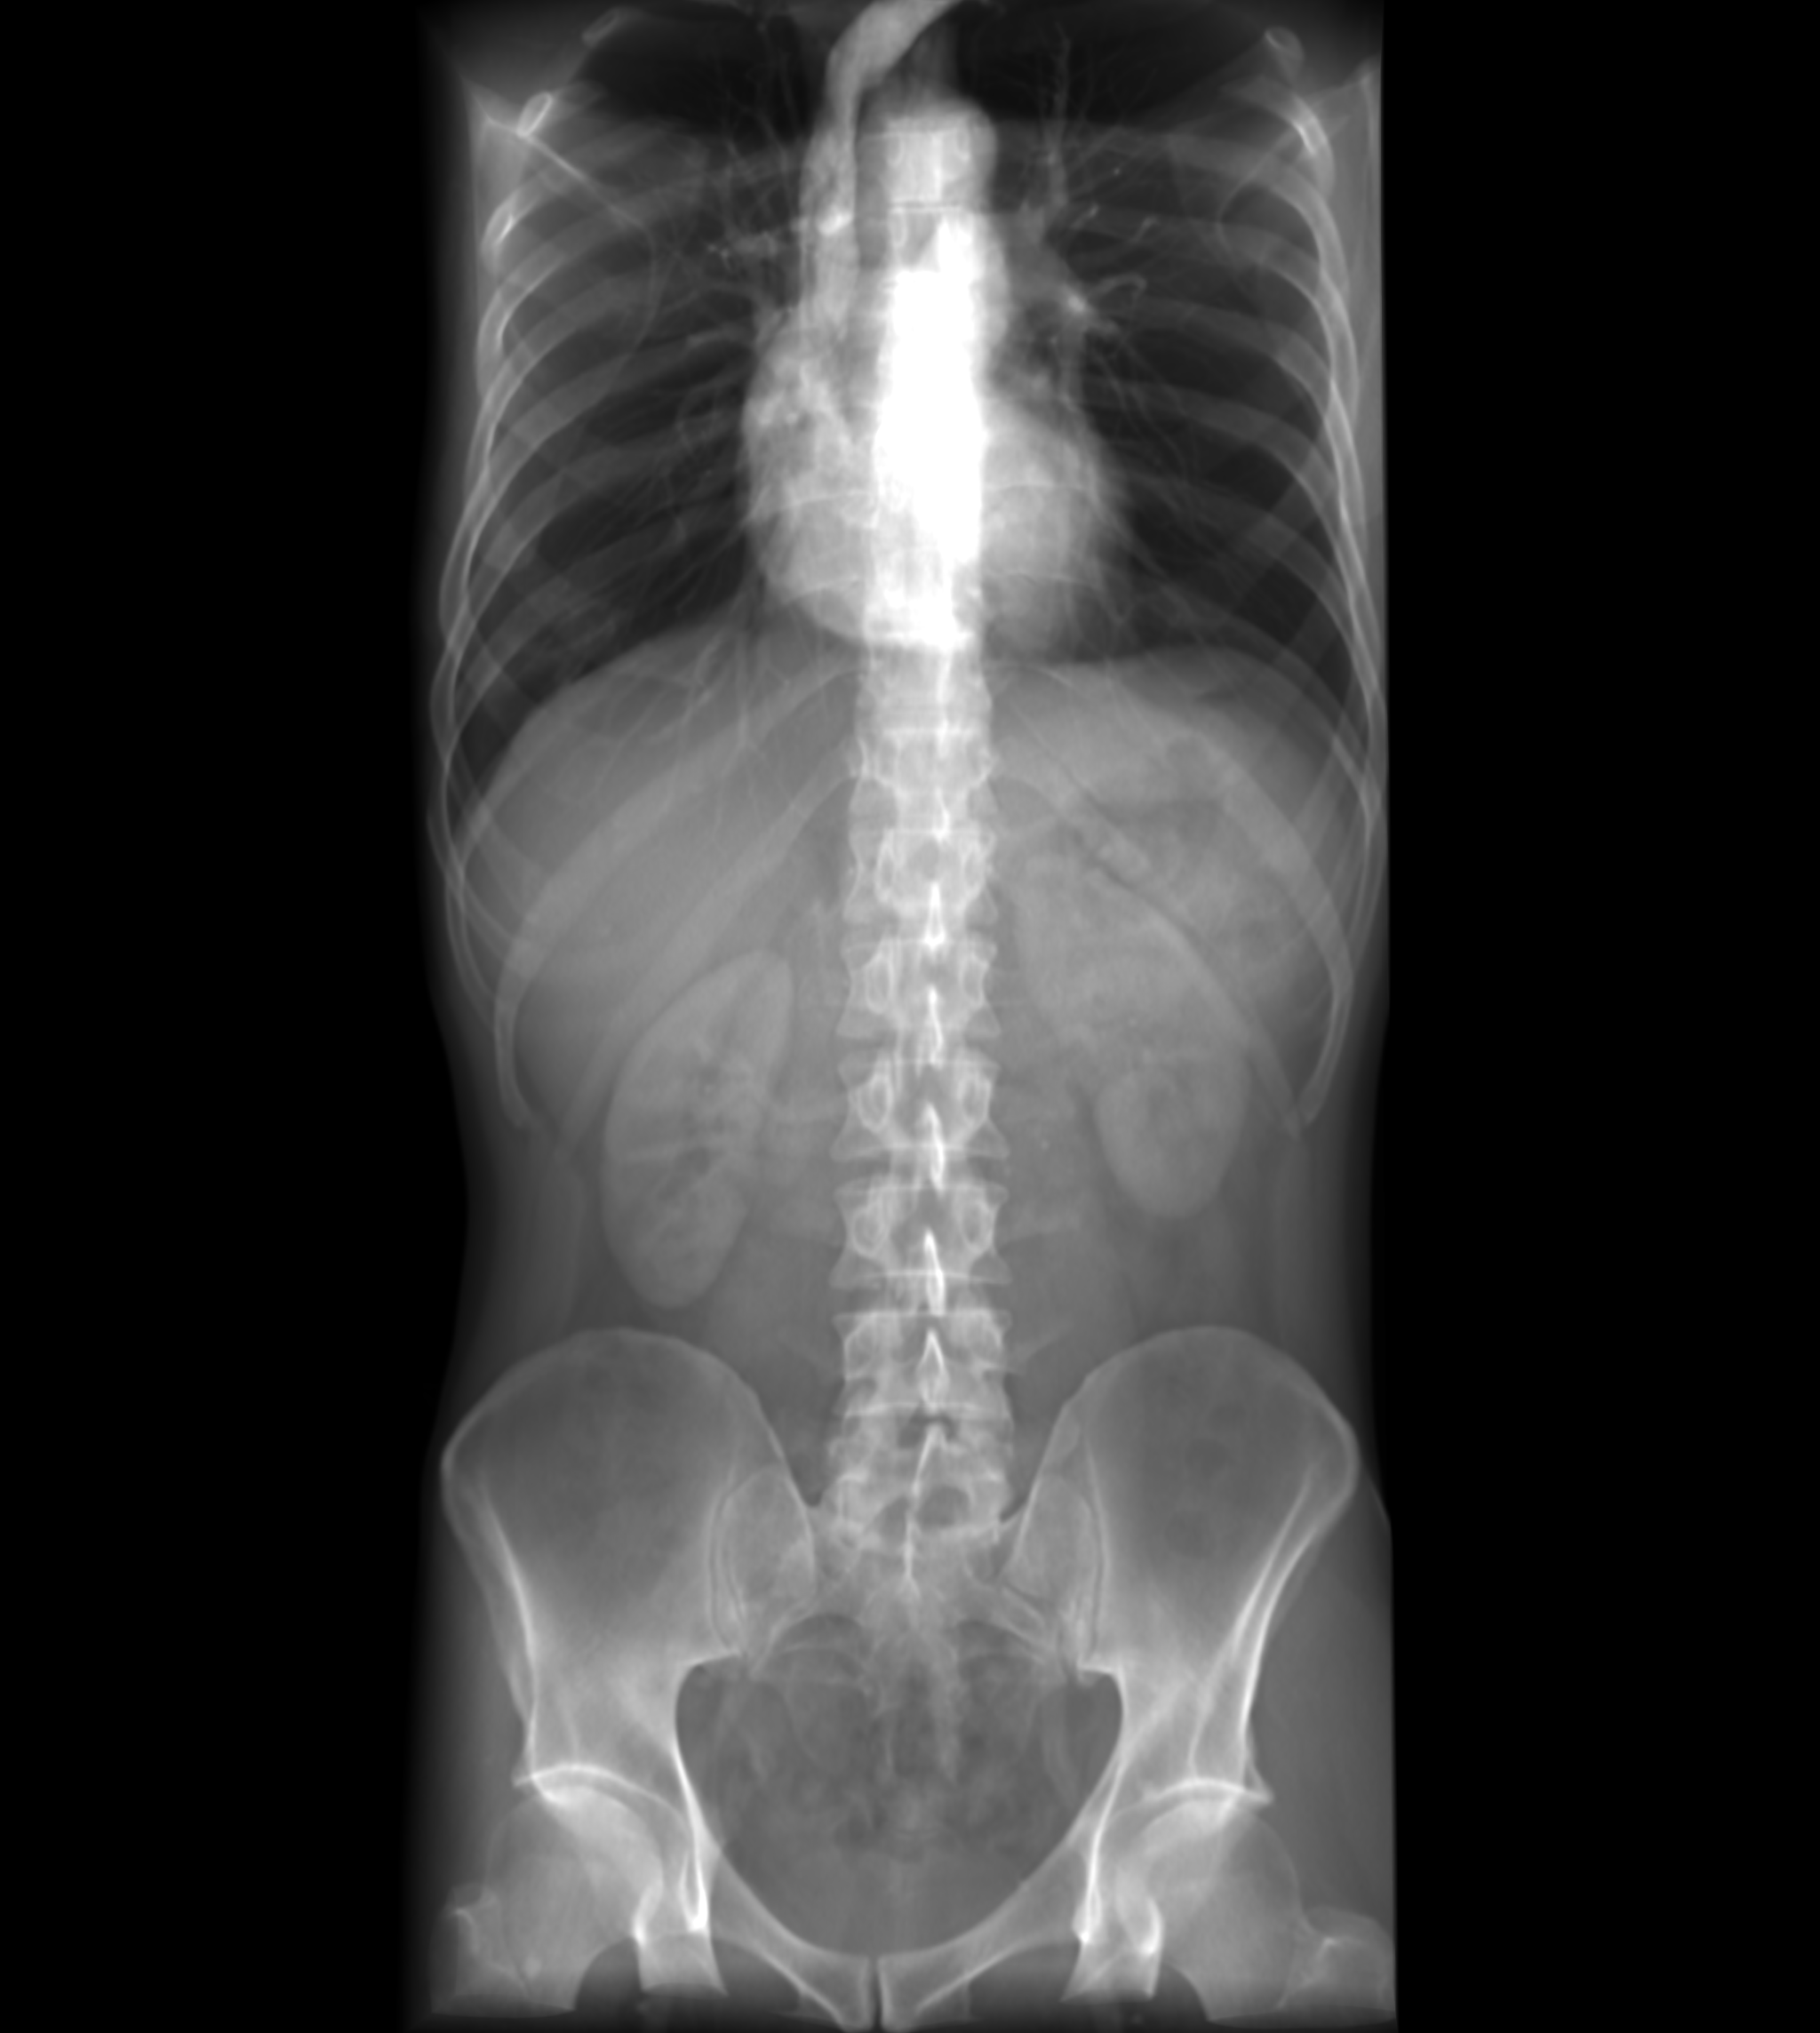
\includegraphics[width=\columnwidth]{TorsoBlendingAdditive}
    \caption{Additive}
    \label{fig:blendadditive}
  \end{subfigure}%
  \begin{subfigure}{.5\columnwidth}
    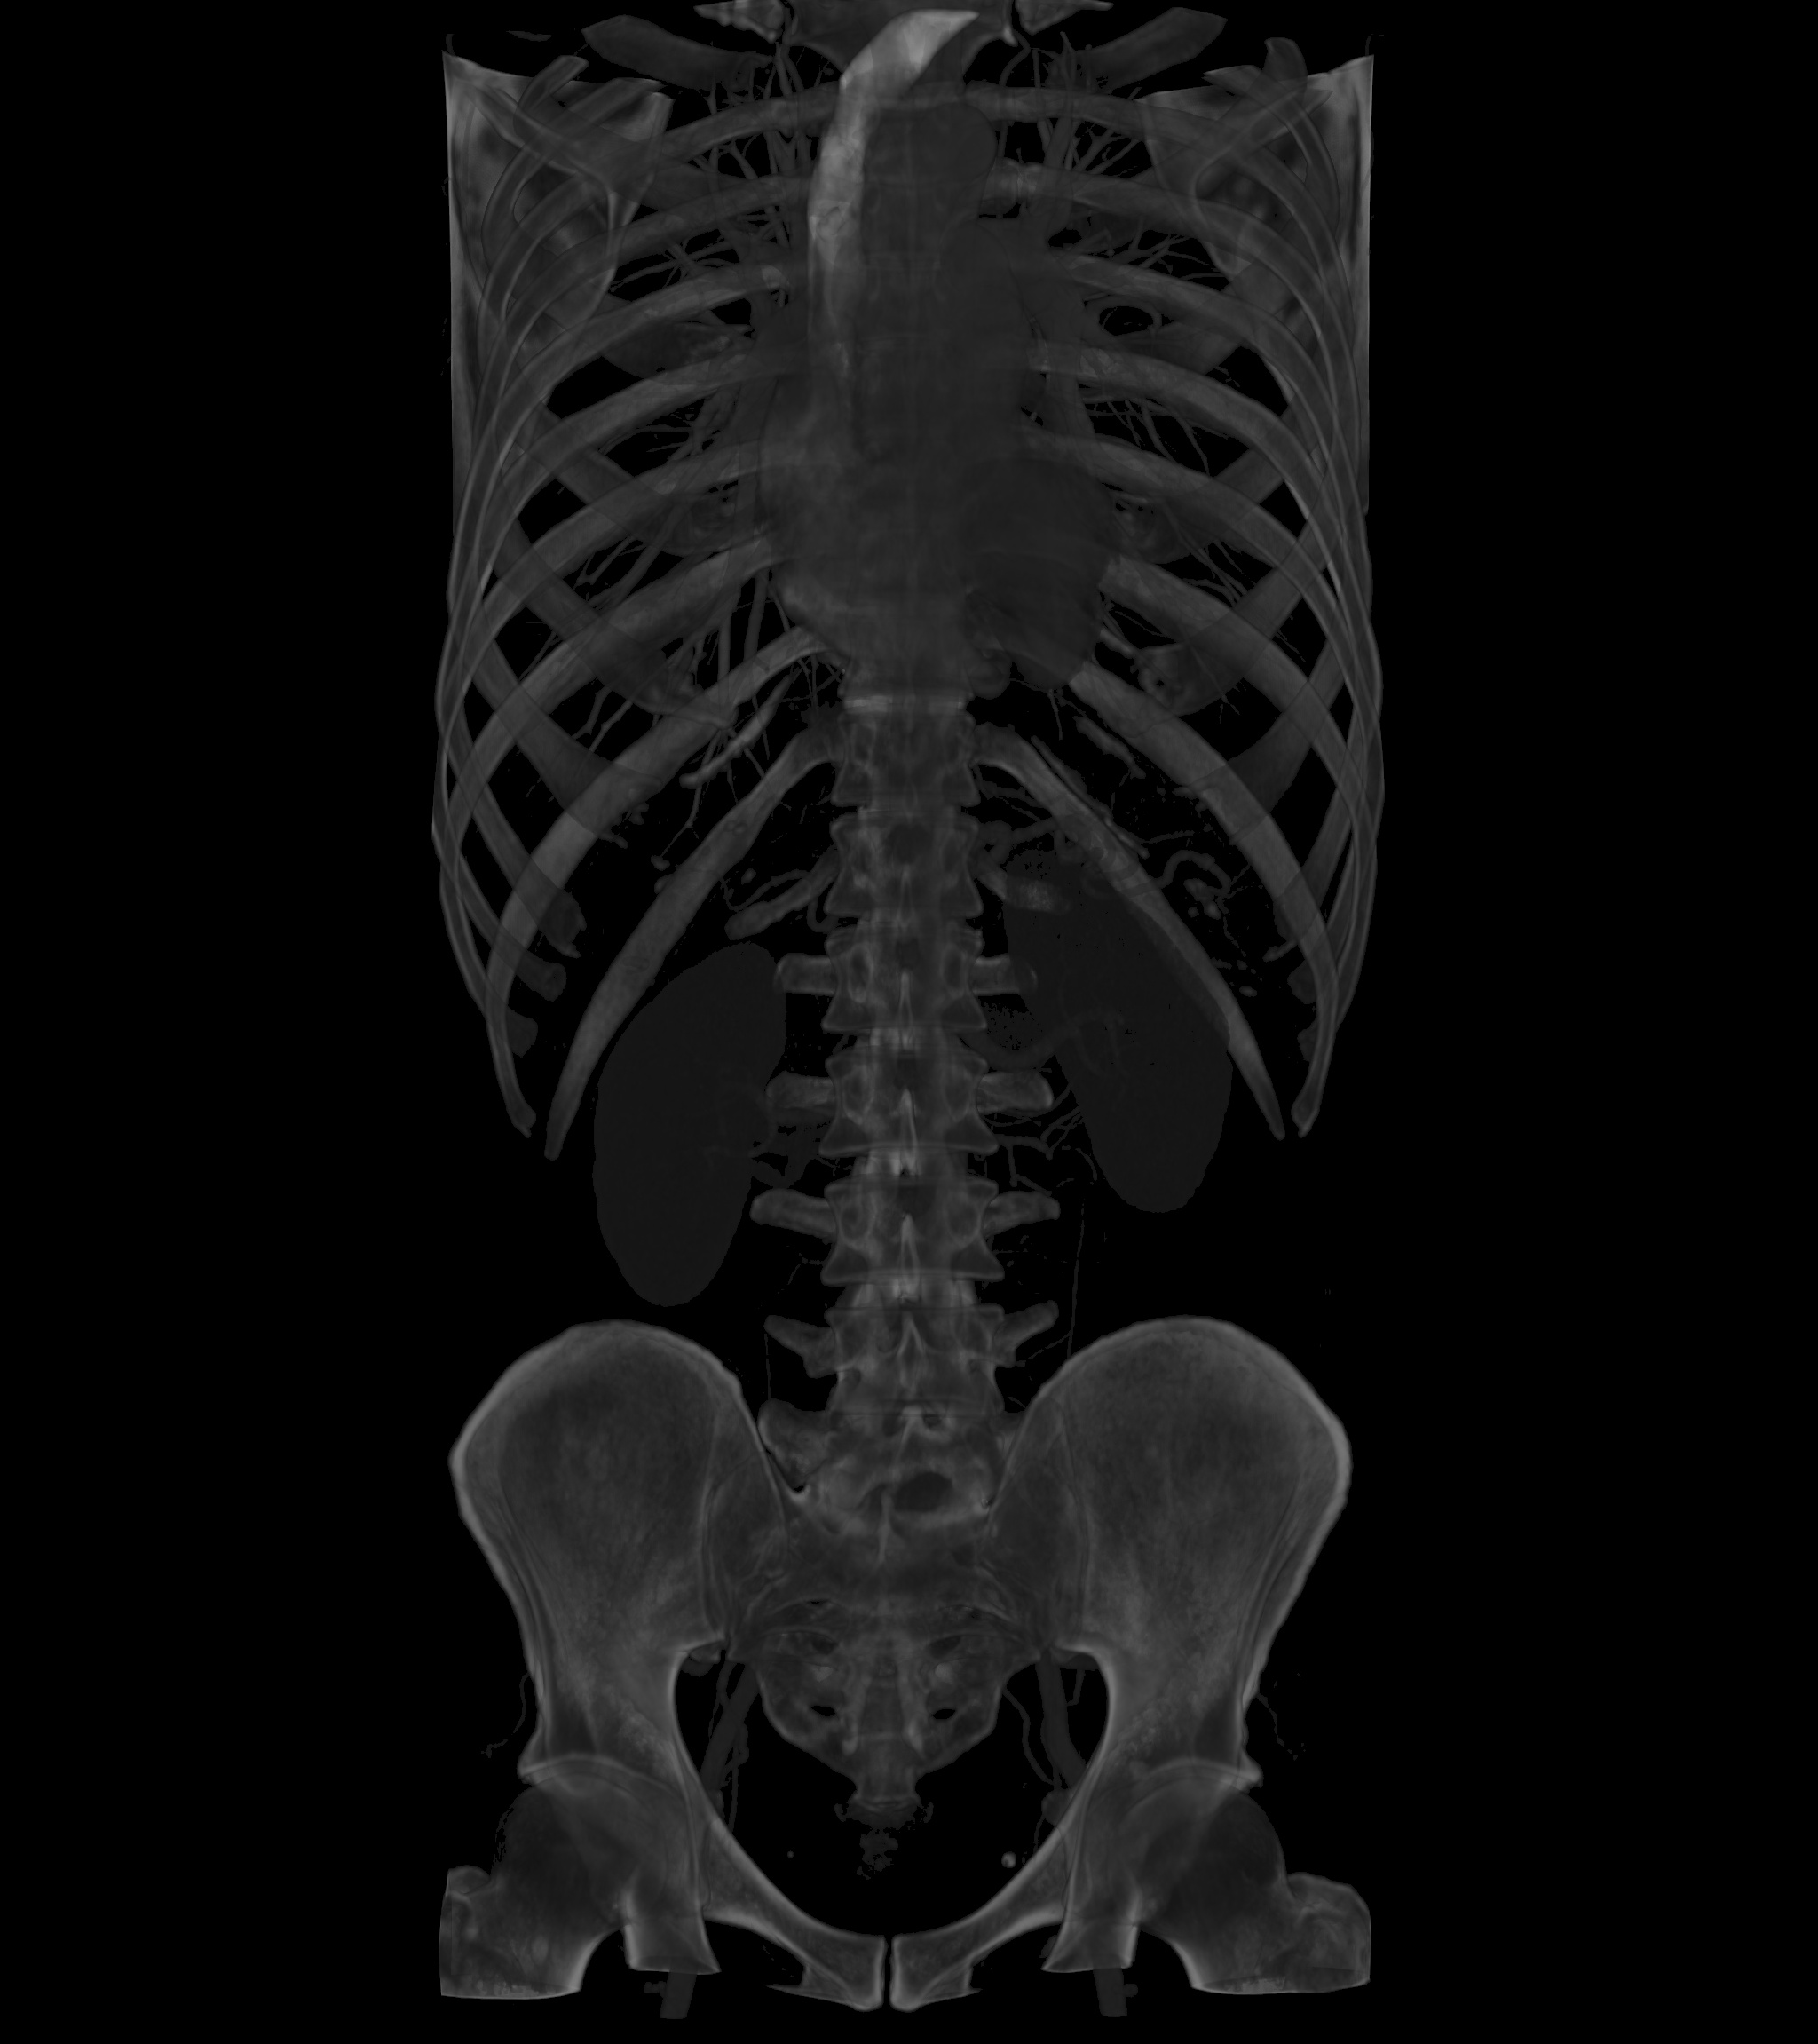
\includegraphics[width=\columnwidth]{TorsoBlendingAverage}
    \caption{Average Intensity}
    \label{fig:blendaverage}
  \end{subfigure}%
  \caption{Blend modes supported by \texttt{vtkGPUVolumeRayCastMapper}}
  \label{fig:blendingmodes}
\end{figure}

\subsection{Masking}
\label{masking}
Both binary and label masks are supported. With binary masks, the value in the
masking volume indicates visibility of the voxel in the data volume. When a
label map is in use, the value in the label map is used to select different
rendering parameters for that sample.  See~\Autoref{fig:rendertotexture}for an
example of label data masks.

\subsection{Opacity Modulated by Gradient Magnitude}
\label{opacity-modulated-by-gradient-magnitude}
While the~\texttt{vtkGPUVolumeRayCastMapper} supports direct accumulation of
color and opacity values along the ray, it also allows for modulating the
opacity accumulation calculation based on relative values of each voxel in the
dataset. Prior efforts~\citep{marchesin_per-pixel_2010} have demonstrated the
usefulness of such a technique for feature enhancement in the rendered image. A
transfer function mapping the magnitude of the gradient to an opacity modulation
value can be used to essentially perform edge detection (de-emphasize homogenous
regions) during rendering. See~\Autoref{fig:gradient} for an example of
rendering with and without the use of a gradient opacity transfer function.

\begin{figure}[htb]
  \centering
   \begin{subfigure}[b]{0.5\columnwidth}
     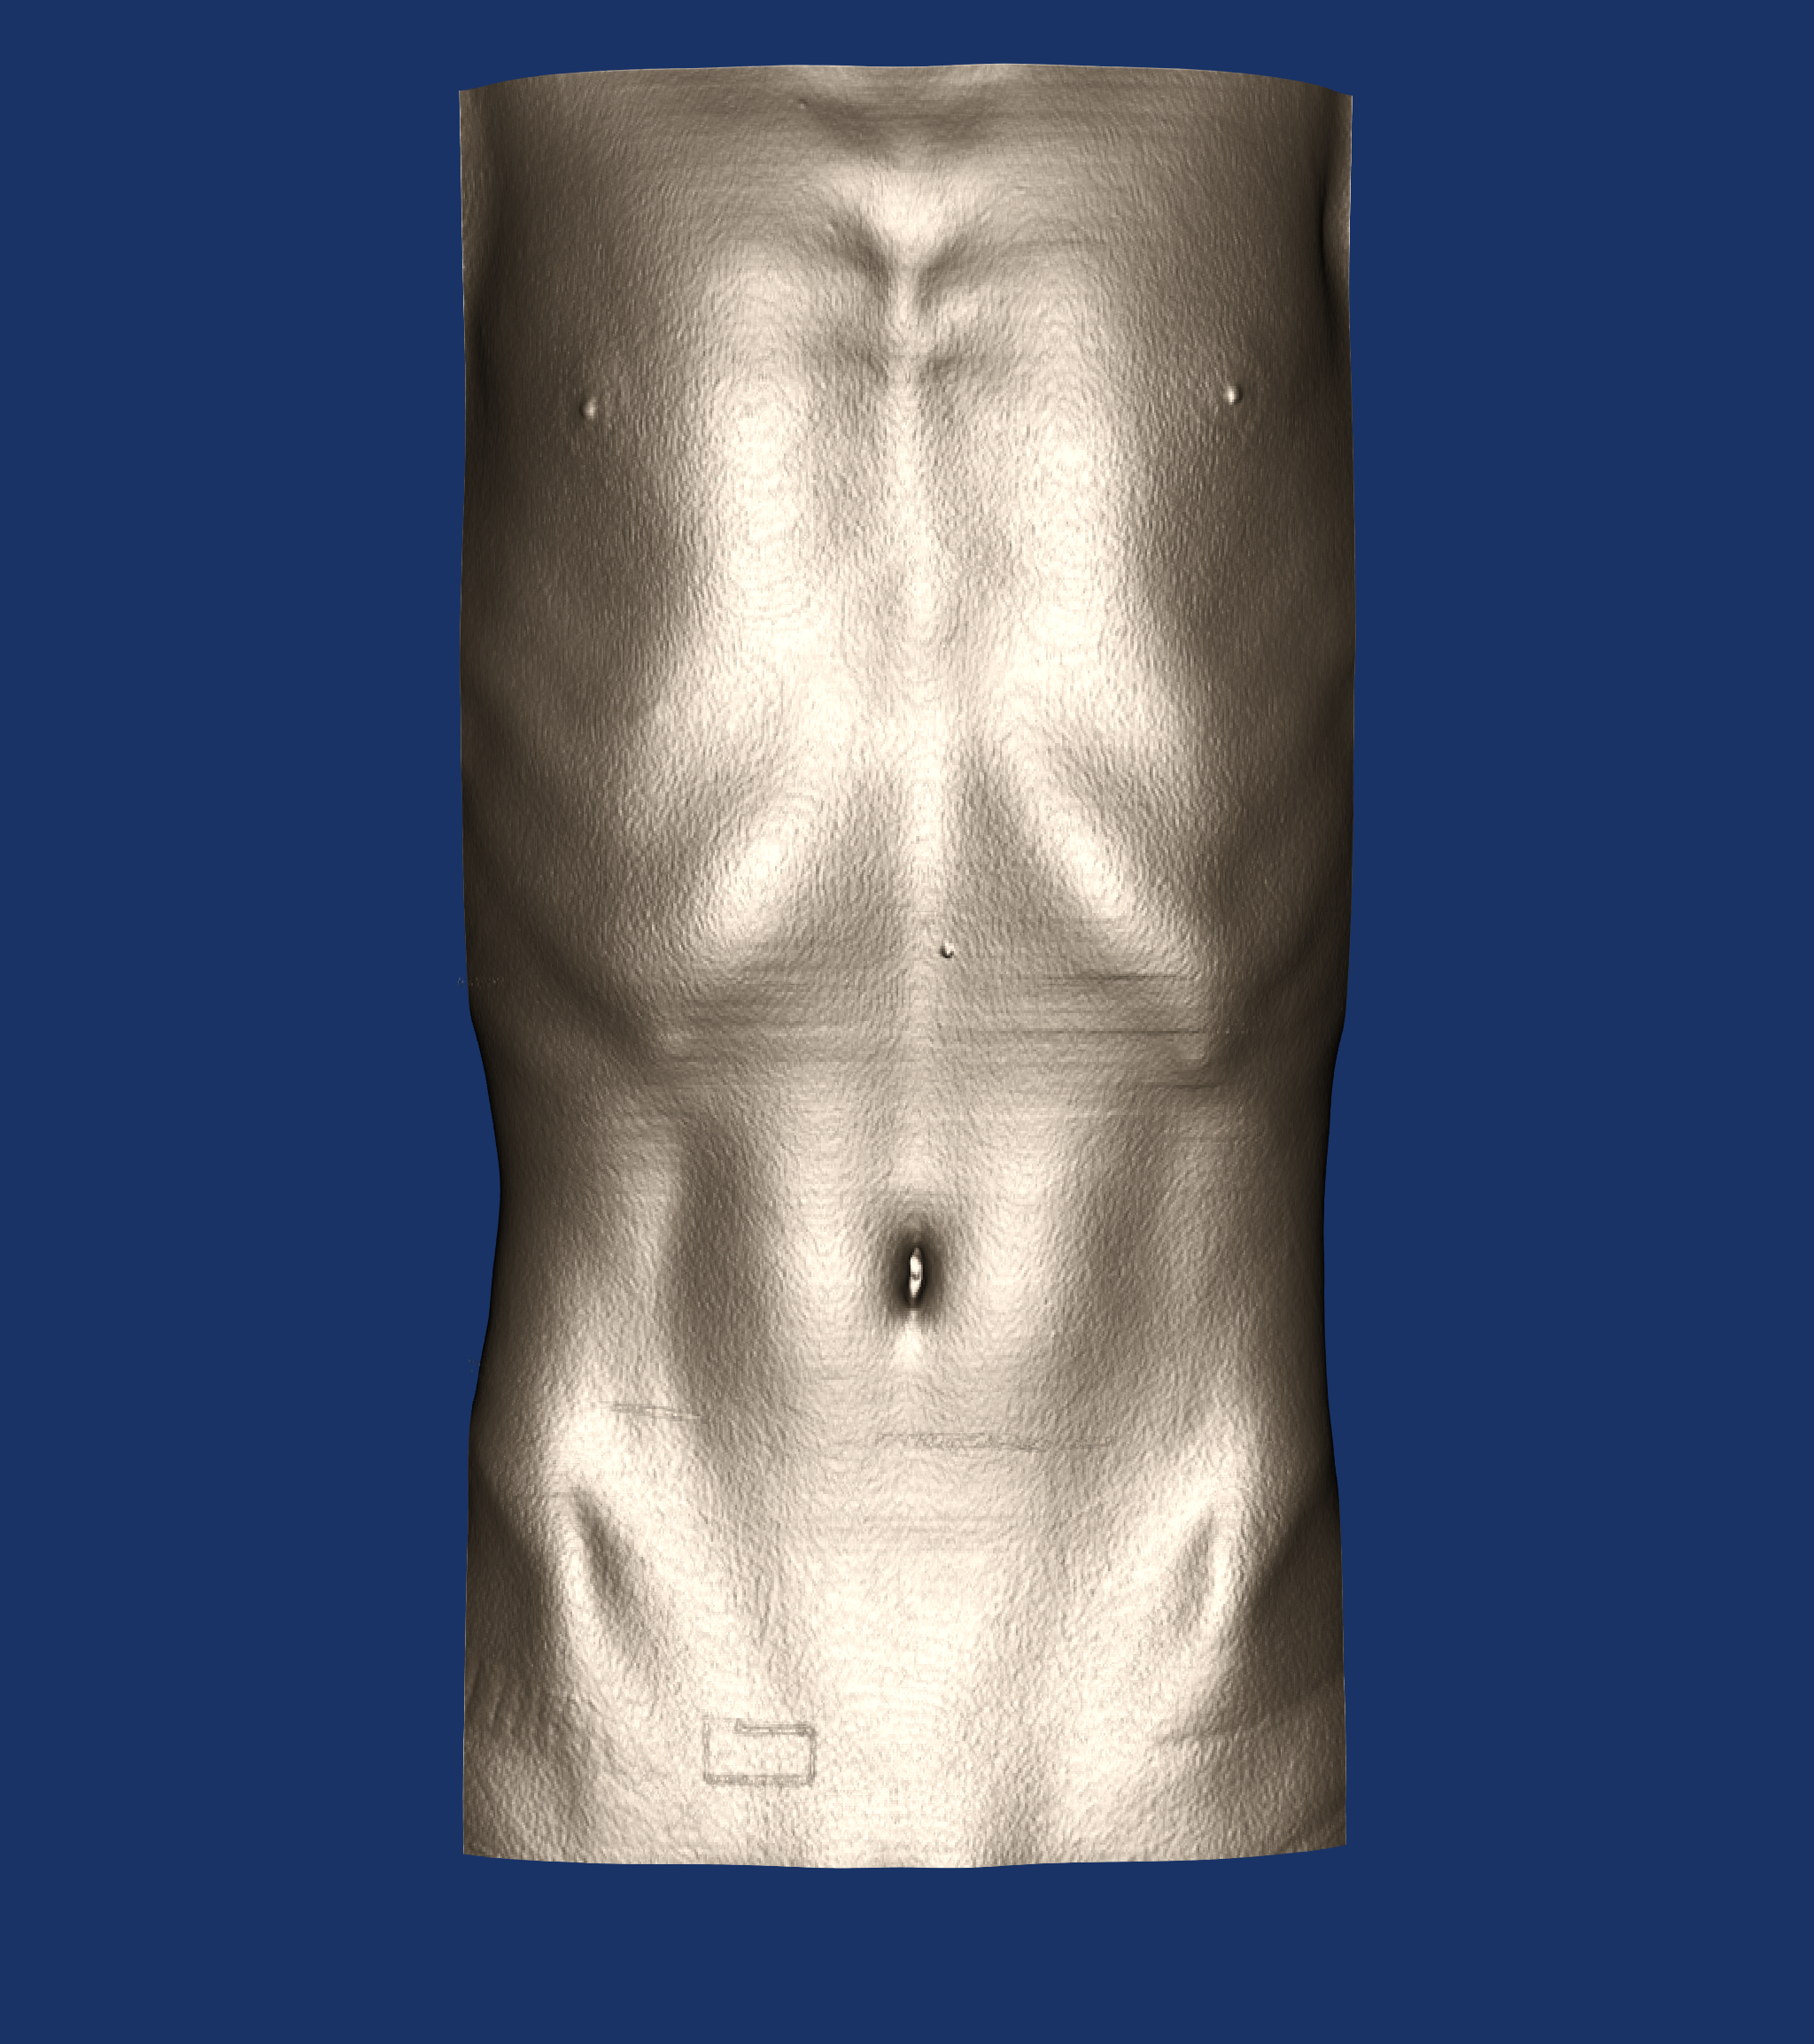
\includegraphics[width=\columnwidth]{TorsoNoGradient}
     \caption{Without gradient opacity}
     \label{fig:Ng1}
   \end{subfigure}%
  \begin{subfigure}[b]{0.5\columnwidth}
    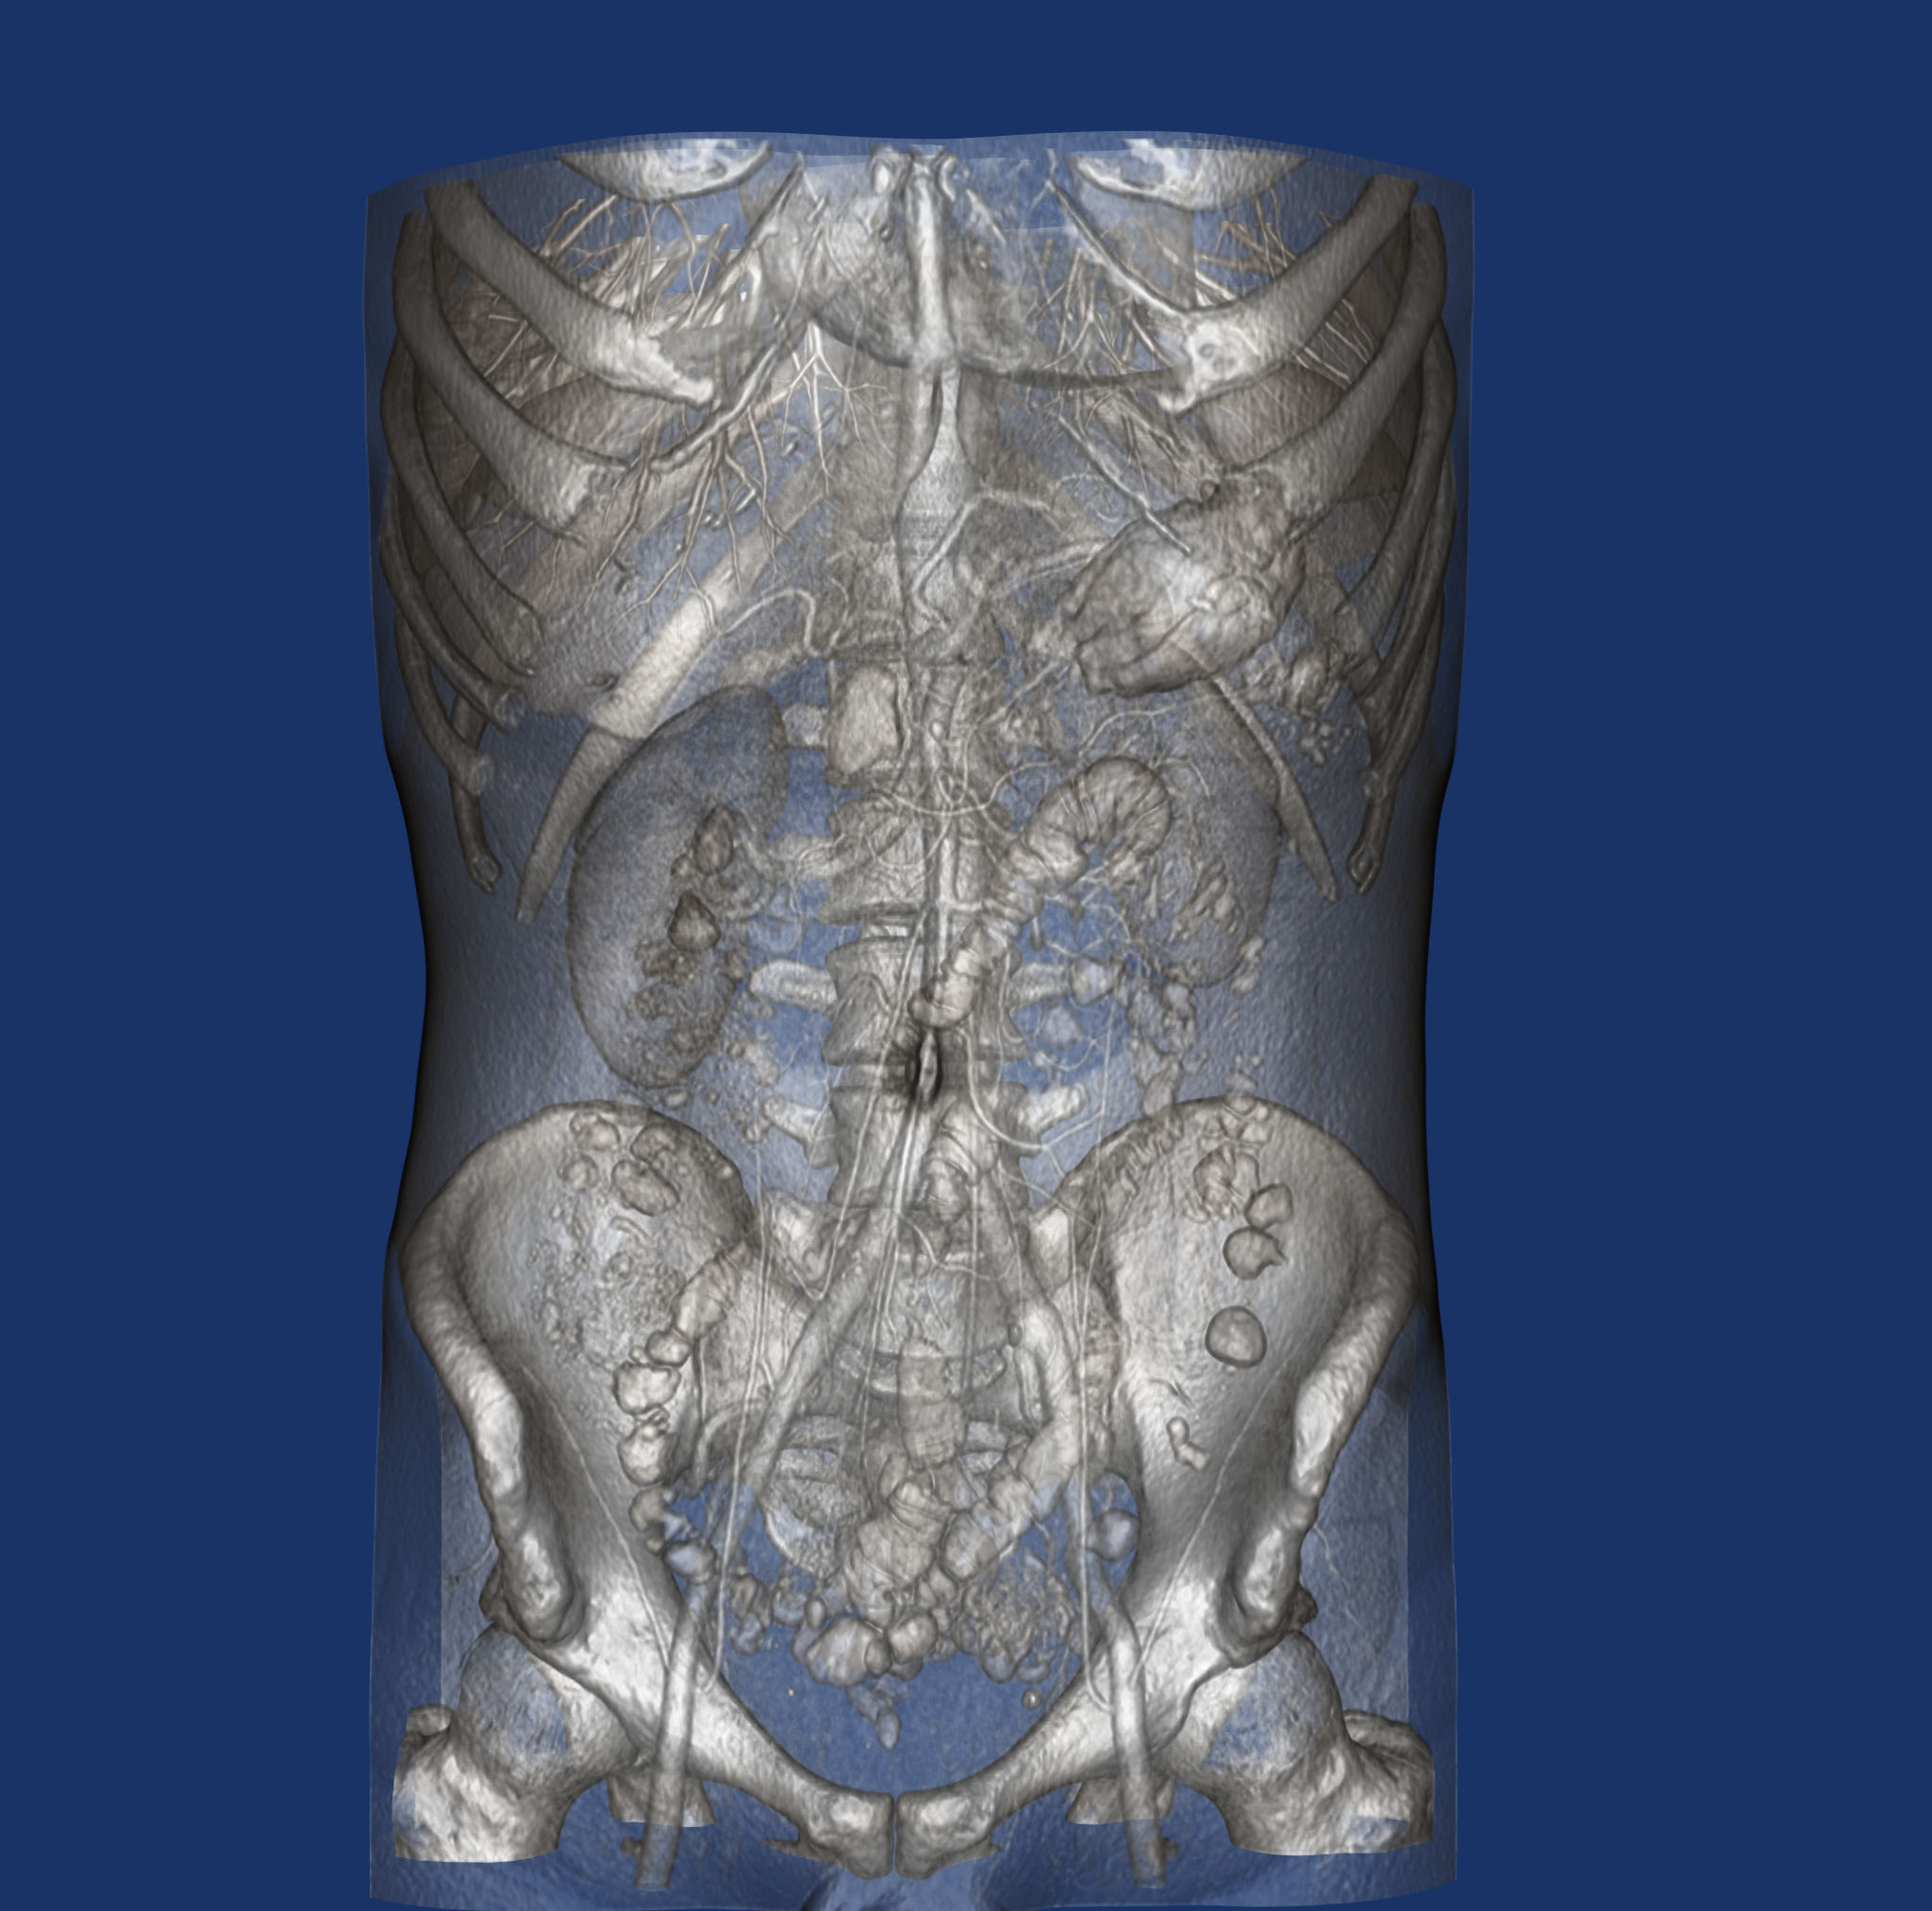
\includegraphics[width=\columnwidth]{TorsoGradient}
    \caption{With gradient opacity}
    \label{fig:Ng2}
  \end{subfigure}
  \caption{Gradient magnitude based opacity modulation}
  \label{fig:gradient}
\end{figure}

\subsection{Optimizations and Edge-Cases} The new
\texttt{vtkOpenGLGPUVolumeRayCastMapper} is more than just a ray cast mapper
implementation. It is designed to work on multiple platforms and developed to
perform volume rendering at interactive frame rates. To achieve interactive
frame rates and to handle edge cases, we have implemented following
optimizations in the new mapper.

\begin{itemize}
  \item \emph{Clipping plane optimization} In VTK a user can place multiple
    planes at desired angles to clip the volume. This technique is essential for
    many medical use-cases. Since only one side of clip planes needs to be
    traversed, performing any sort of ray cast on the clipped side is wasteful.
    Hence a simple optimization is to move the starting point of the ray on the
    plane by projecting the ray onto the plane in the view direction.
  \item \emph{Camera Inside the Bounding Box} Rendering with camera views within
    the volume is handled by clipping the proxy geometry with the camera near
    plane (using \texttt{vtkClipConvexPolyData}), thus ensuring that all
    bounding box fragments fall within range.  Plane-Axis-Aligned-Bounding-Box
    intersection is used to determine whether geometry clipping is necessary.
  \item \emph{Support for Double and Long Long Data Type} The current OpenGL API
    does not support 64-bit data types. In order to be able to render volumes of
    these types, the mapper loads the data array slice by slice casting the data
    values to floating-point. This, despite the obvious precision loss, is
    provided to the user as a convenience feature.
\end{itemize}

\section{Performance benchmarks}
\label{performance-benchmarks}
As part of the modernization effort, we obtained several performance metrics
from sample systems with differing specifications of hardware graphics ranging
from on-board graphic cards to dedicated GPUs. The code used for benchmarking is
located within the VTK code repository under \texttt{Utilities/Benchmarks/}. The
test runs for a specified number of iterations with each iteration increasing
data size. For each iteration, the test creates a mock dataset using
the~\texttt{vtkRTAnalyticSource} and renders it for 80 frames, rotating the
dataset each frame and recording the time taken to render to screen.  Each test
was run twice on each system; once with and once without gradient computations
required by shading.

The results of the benchmarking are shown in~\Autoref{fig:perf-bench}. As observed,
surface shaded rendering degrades performance but the mapper maintains
interactive frame rates even for large datasets. Note that the tests on some
systems were restricted to a maximum voxel count of 300 million voxels owing to
graphics memory limitations. Note also that we were able to render large volumes
requiring more than the available graphics memory using texture streaming, as
described in~\Autoref{streaming}, outside the scope of this performance
benchmark evaluation.

\begin{figure}[ht]
  \centering
  \begin{tikzpicture}
    \begin{groupplot}[
      group style = {
        group name=benchmarks,
        group size=1 by 2,
        xlabels at=edge bottom,
        xticklabels at=edge bottom
      },
      width=\linewidth,
      xlabel=Number of voxels in data (x 1 Million),
      label style={font=\footnotesize},
      tick label style={font=\footnotesize},
      xmode=log,
      xmin=9,
      xmax=2100,
      ymin=-10,
      ylabel=Frames per second,
      grid=both,
      grid style={line width=.1pt, draw=gray!10},
      legend pos=north east,
      legend style={font=\fontsize{4}{5}\selectfont}
      ]
    %\begin{axis}[
      %width = \linewidth,
      %xlabel=Number of voxels in data (x 1 Million),
      %xmode=log,
      %ylabel=Frames per second,
      %grid=both,
      %grid style={line width=.1pt, draw=gray!10}
      %]
      \nextgroupplot
      \addlegendimage{empty legend}
      \addlegendentry{\hspace{-.6cm}\textbf{Without Shading}}
      \addplot[color={rgb:red,228;green,26;blue,28},mark=10-pointed star] file {data/k5200.txt};
      \label{plot_k52}
      \addlegendentry{NVIDIA Quadro K5200}
      \addplot[color={rgb:red,77;blue,175;green,74},mark=otimes] file {data/amdD300.txt};
      \label{plot_a3}
      \addlegendentry{AMD FirePro D300}
      \addplot[color={rgb:red,101;blue,10;green,64},mark=star] file {data/geforce960M.txt};
      \label{plot_gf96}
      \addlegendentry{NVIDIA GeForce 960M}
      \addplot[color={rgb:red,55;green,126;blue,184},mark=o] file {data/iris.txt};
      \label{plot_iris}
      \addlegendentry{Intel Iris Graphics 550}
      \addplot[color={rgb:red,255;blue,255;green,51},mark=triangle*] file {data/quadro2000.txt};
      \label{plot_q20}
      \addlegendentry{NVIDIA Quadro 2000}
      \addplot[color={rgb:red,152;blue,78;green,163},mark=diamond] file {data/intelhd530.txt};
      \label{plot_i530}
      \addlegendentry{Intel Graphics HD 530}
      
      \nextgroupplot
      \addlegendimage{empty legend}
      \addlegendentry{\hspace{-.6cm}\textbf{With Shading}}
      \addplot[color={rgb:red,228;green,26;blue,28},mark=10-pointed star] file {data/k5200_shaded.txt};
      \label{plot_k52_s}
      \addlegendentry{NVIDIA Quadro K5200}
      \addplot[color={rgb:red,77;blue,175;green,74},mark=otimes] file {data/amdD300_shaded.txt};
      \label{plot_a3_s}
      \addlegendentry{AMD FirePro D300}
      \addplot[color={rgb:red,101;blue,10;green,64},mark=star] file {data/geforce960M_shaded.txt};
      \label{plot_gf96_s}
      \addlegendentry{NVIDIA GeForce 960M}
      \addplot[color={rgb:red,55;green,126;blue,184},mark=o] file {data/iris_shaded.txt};
      \label{plot_iris_s}
      \addlegendentry{Intel Iris Graphics 550}
      \addplot[color={rgb:red,255;blue,255;green,51},mark=triangle*] file {data/quadro2000_shaded.txt};
      \label{plot_q20_s}
      \addlegendentry{NVIDIA Quadro 2000}
      \addplot[color={rgb:red,152;blue,78;green,163},mark=diamond] file {data/intelhd530_shaded.txt};
      \label{plot_i530_s}
      \addlegendentry{Intel Graphics HD 530}
    \end{groupplot}
    %legend
    %\node [draw,fill=white] at (rel axis cs: 0.4,0.9) {
      %\shortstack[l]{
        %\tiny{\textbf{Without Shading}} \\
        %\ref{plot_k52} \tiny{NVIDIA Quadro K5200} \\
        %\ref{plot_a3} \tiny{AMD FirePro D300}\\
        %\ref{plot_q20} \tiny{NVIDIA Quadro 2000}\\
        %\ref{plot_gf96} \tiny{NVIDIA GeForce 960M}\\
        %\ref{plot_i530} \tiny{Intel Graphics HD 530}\\
        %\ref{plot_iris} \tiny{Intel Iris Graphics 550}
      %}};
    %\node [draw,fill=white] at (rel axis cs: 0.4,-0.4) {
      %\shortstack[l]{
        %\tiny{\textbf{With Shading}} \\
        %\ref{plot_k52_s} \tiny{NVIDIA Quadro K5200}\\
        %\ref{plot_a3_s} \tiny{AMD FirePro D300}\\
        %\ref{plot_q20_s} \tiny{NVIDIA Quadro 2000}\\
        %\ref{plot_gf96_s} \tiny{NVIDIA GeForce 960M}\\
        %\ref{plot_i530_s} \tiny{Intel Graphics HD 530}\\
        %\ref{plot_iris_s} \tiny{Intel Iris Graphics 550}
      %}};
  \end{tikzpicture}
  \caption{Results of the benchmarking tests performed on six different
    graphics cards using the~\protect{\texttt{vtkGPUVolumeRayCastMapper}}
    without and with surface shading (i.e. gradient computations)}
  \label{fig:perf-bench}
\end{figure}

\section{Application Areas}
\label{applicationareas}

One of the goals of our work is to support volume visualization for various
domains (scientific, medical), on multiple devices (workstations, virtual
reality, mobile, clusters) and on different operating systems (Linux, Mac,
Windows). This is important as VTK is used by a large user base in different
setups.  In the next few sub-sections, we have presented improvements to our
mapper for different domains and environments.

\subsection{Domains}
\label{domains}

Owing to the fact that the new mapper is built with the VTK pipeline model
(see~\Autoref{fig:pipeline}), it can be integrated into existing VTK
applications with little effort. As described
in~\Autoref{implementationdetails}, the volume mapper provides a rich
feature-set for a rendering a variety of data types. This versatility allows the
mapper to be used in diverse scientific and medical domains for volumetric
visualization. As shown in~\Autoref{fig:paraview-turbulent-combustion,
fig:tomviz-cop}, the mapper has found its way into real-world scientific
applications like ParaView~\citep{ahrens_paraview:_2005, ayachit_paraview_2015,
ayachit_paraview_2015-1} and tomviz~\citep{hanwell_tomviz_2014}. The volume
mapper can be used for
visualizing data generated from physics simulations (~\Autoref{fig:supernova}),
transmission and scanning transmission electron microscopes
(~\Autoref{fig:ptcu-grad}) and medical and dental CT scans
(~\Autoref{fig:volume_peeling_tooth, fig:blendingmodes, fig:clipping}). 

\begin{figure}[ht]
  \begin{subfigure}[b]{0.49\columnwidth}
    %\centering
    \includegraphics[width=\textwidth]{SMALL-PtCu-NP-Grad.png}
    \caption{Platinum-Copper~(\ce{PtCu})
      nanoparticle \protect\citep{scott_electron_2012, miao_atomic_2016} with
      gradient opacity modulation enabled}
    \label{fig:ptcu-grad}
  \end{subfigure}\hfill%
  \begin{subfigure}[b]{0.49\columnwidth}
    %\centering
    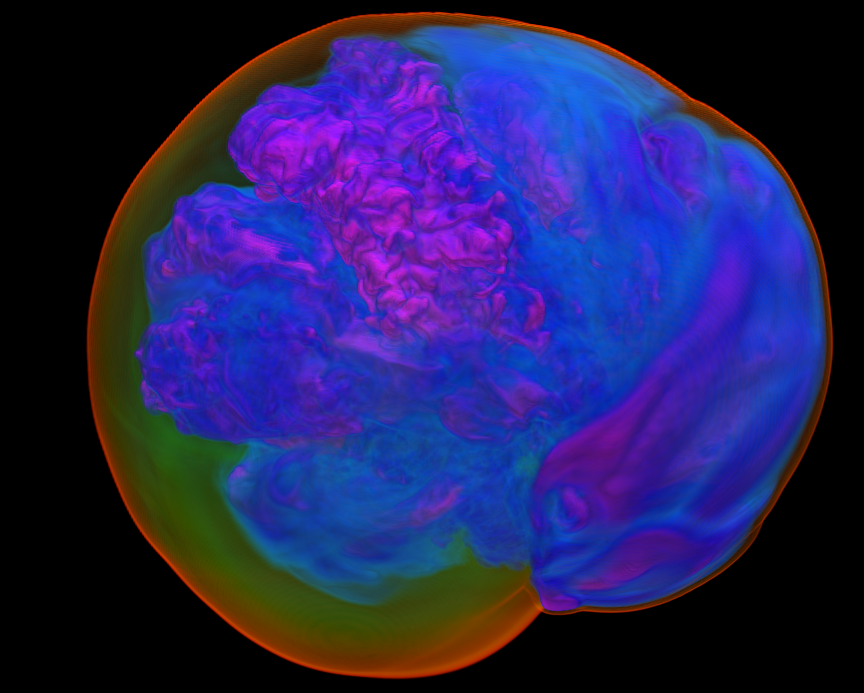
\includegraphics[width=\textwidth]{supernova-simulation.png}
    \caption{Rendering a single timestep output of the supernova modeling
      simulation~\protect\citep{blondin_pulsar_2007}}
    \label{fig:supernova}
  \end{subfigure}
  \caption{Physics and chemistry data visualization using
    the~\texttt{vtkGPUVolumeRayCastMapper}}
  \label{fig:domains}
\end{figure}

\begin{figure}[ht]
  \centering
  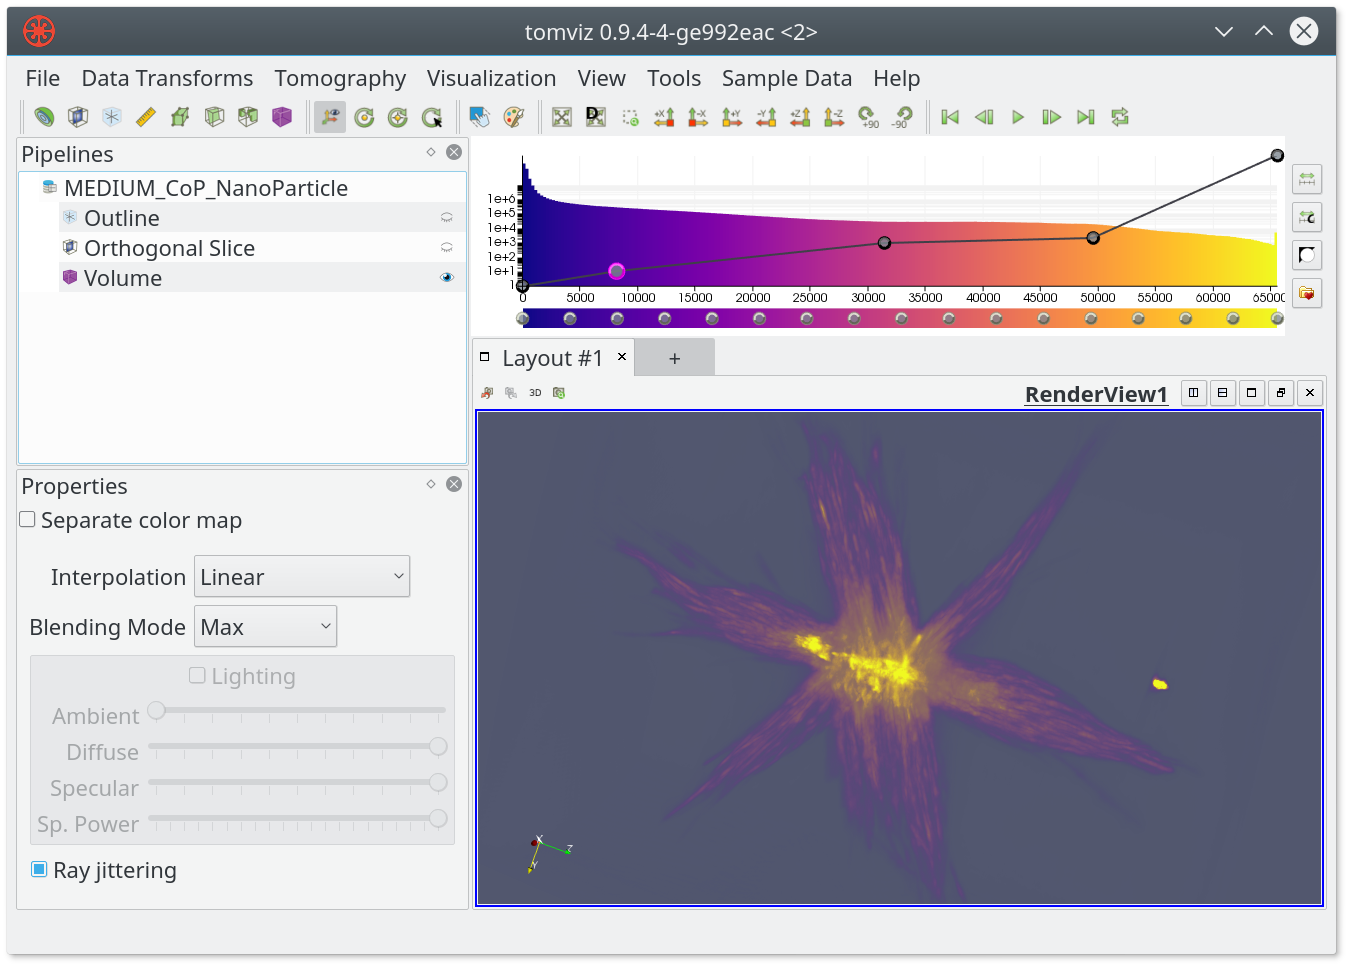
\includegraphics[width=\columnwidth]{tomviz-medium-CoP.png}
  \caption{Tomviz~\protect\citep{hanwell_tomviz_2014} rendering a
    Cobalt-Phosphorous (\ce{Co2P})
    nanoparticle~\protect\citep{levin_nanomaterial_2016}}
  \label{fig:tomviz-cop}
\end{figure}

\begin{figure}[ht]
  \centering
  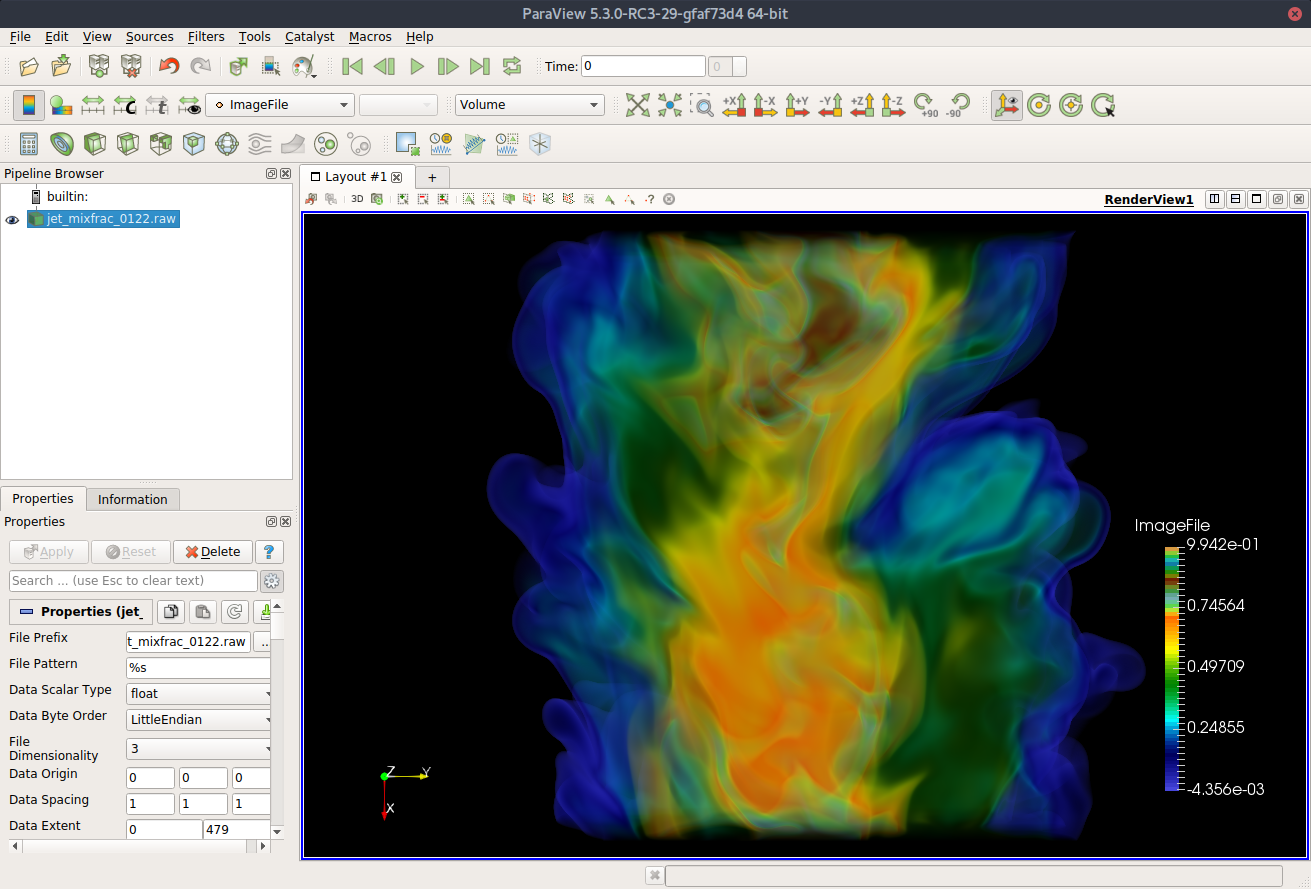
\includegraphics[width=\columnwidth]{paraview-turbulent-combustion-simulation.png}
  \caption{ParaView~\protect\citep{ahrens_paraview:_2005, ayachit_paraview_2015,
  ayachit_paraview_2015-1} rendering a single time step of a simulation of
  temporally-evolving plane jet
  flames~\protect\citep{hiroshi_akiba_visualizing_2007}}
  \label{fig:paraview-turbulent-combustion}
\end{figure}

\subsection{Devices and Environments}
\label{devices-and-environments}
The new volume mapper supports rendering on most common devices including mobile
platforms.  This poses a challenge as the mapper would have to be versatile
enough to handle low computing power requirements of mobile devices and scene
composition in a multi-processor cluster environment simultaneously and still
perform at~\textit{interactive} frame rates. 

\subsubsection{Mobile Support}
\label{mobile}
The decision to use OpenGL 3 or higher enabled volume rendering to support
mobile devices (iOS and Android devices) since OpenGL ES 3.0 supports 3D textures.
However OpenGL ES does not support all of the texture format types, therefore,
new texture formats are added with compile time switches to enable or
disable them depending on whether the platform is desktop or mobile. One such
example is capturing of depth buffer since that is not yet supported on the
mobile platform.  Furthermore, as interactions on mobile devices require touch
interactions, the new rendering system added support for multi-touch events
such as using two fingers to translate, rotate, and zoom the camera. With minor
feature-set exceptions, the new volume mapper works on mobile devices enabling
developers to build sophisticated applications for the scientific community.

Various artifacts arise when rendering parallely (bricking) on a cluster.
Artifacts due to sampling, gradient computation, etc.  are seen at the edges of
each of the bricks.  To address it, our mapper ensures the entry texture
coordinate and the limit texture coordinates are correctly adjusted to, and the
ray step is scaled accordingly.

Finally, to perform consistently across various devices, our mapper uses two
critical pieces of information from VTK. First, the last frame-render time, and
second, the desired frame rate for the application. Using these two factors, the
mapper distinguishes between an~\textit{interactive} versus~\textit{still}
render and accordingly makes adjustments to the ray sampling computations to
achieve the desired frame rate. 

\section{Future Work}
\label{future-work}
At this point, we have a replacement class for vtkGPURayCastMapper that is more
widely supported, faster, more easily extensible, and supports majority of the
features of the old class. In the near future, our goal is to ensure that this
mapper works as promised by integrating it into existing VTK applications such
as ParaView and Slicer. Once these tasks are complete, we have some ideas on new
features we would like to add to this mapper (outlined below).

\subsection{2D Transfer Functions}
\label{2d-transfer-functions}
Currently, volume rendering in VTK uses three independent 1D transfer functions
to map scalar value to color, scalar value to opacity and gradient magnitude to
opacity. Increasing the number of parameters in a transfer function can improve
discrimination between structures in the volume data given that the combined
parametric information allows to disambiguate areas that fall within a given range
of those parameters simultaneously. Enhanced structure discrimination is beneficial
in medical image visualization where distinct tissues are approximately constant
in value and values transition smoothly from one tissue to the next. There is on-going
work to support 2D transfer functions combining scalar value and gradient magnitude
(the scalar field variable and its first derivative) under the the DOE Office of
Science contract DE-SC0011385 grant.

\subsection{Overlapping Volumes}
\label{overlapping-volumes}
It is currently possible to render overlapping volumes by taking advantage of
the up to 4 independent components supported by the mapper (each component
representing a different volume).
The limitation with this approach is that each of the overlapping volumes are
required to be sampled in the same grid, hence all of the volumes are required
to share the same dimensions.  Nonetheless, in order to extend the mapper to
support overlapping volumes sampled in grids with different dimensions, rays
should be casted through proxy geometry bounding the N overlapping volumes to be
rendered and separately sampling and compositing their fetched texture values in
the fragment shader.

\subsection{Improved Rendering of Labeled Data}
\label{improved-rendering-of-labeled-data}
Currently, VTK supports binary masks and only a couple of very specific versions
of label mapping. We know that our community needs more extensive label mapping
functionality – especially for medical datasets. Labeled data requires careful
attention to the interpolation method used for various parameters. (You may wish
to use linear interpolation for the scalar value to look up opacity, but,
perhaps, select the nearest label to look up the color.) We
plan to solicit feedback from the VTK community to understand the sources of
labeled data and the application requirements for visualization of this data. We
then hope to implement more comprehensive labeled data volume rendering for both
the CPU and GPU mappers.

\section{Acknowledgements}
\label{acknowledgements}
We would like to recognize the National Institutes of Health for sponsoring this
work under the grant NIH R01EB014955 - ``Accelerating Community-Driven Medical
Innovation with VTK.'' 

We thank the maintainers of the OsiriX DICOM Image
Library~\citep{osirix_osirix_2017} for providing the head (used
in~\Autoref{fig:clipping}) and torso (used in~\Autoref{fig:rendertotexture,
fig:blendingmodes, fig:gradient}) datasets used in this publication. The
Supernova (used for ~\Autoref{fig:supernova}) and Turbulent-Combustion (used
for~\Autoref{fig:paraview-turbulent-combustion}) datasets were obtained from
VisFiles~\citep{visfiles_visfiles_2007}. The supernova dataset is made available
by John Blondin at the North Carolina State University through US Department
of Energy's SciDAC Institute for Ultrascale Visualization.The turbulent
combustion dataset is made available by Jackqueline Chen at Sandia
Laboratories through US Department of Energy's SciDAC Institute for Ultrascale
Visualization. We would also like to thank Jianwei (John) Miao from University
of California at Los Angeles and Robert Hovden from Cornell University for
granting us permission to use the~\ce{PtCu} (used in~\Autoref{fig:ptcu-grad})
and~\ce{Co2P} (used in~\Autoref{fig:tomviz-cop}) nanoparticle datasets. The
cactus sample dataset (used in~\Autoref{fig:jittering}) is courtesy of Michael
Holland and Dula Parkinson from Advanced Light Source, Lawrence Berkeley National
Laboratory.


%% References:
\section{References}
\label{}
\bibliography{VTKVR}

\end{document}
\endinput
%%
%% End of file `SoftwareX_article_template.tex'.
